\documentclass{report}

% Uncomment the following line to allow the usage of graphics (.jpg, .png, etc.)
%\usepackage[pdftex]{graphicx}

% Comment the following line to deny the usage of umlauts and other non-ASCII characters
\usepackage[utf8]{inputenc}
\usepackage{marginnote} % Required for margin notes
\usepackage{wallpaper} % Required to set each page to have a background
\usepackage{lastpage} % Required to print the total number of pages
\usepackage[left=1.3cm,right=4.6cm,top=1.8cm,bottom=4.0cm,marginparwidth=3.4cm]{geometry} % Adjust page margins
\usepackage{amsmath} % Required for equation customization
\usepackage{amssymb} % Required to include mathematical symbols
\usepackage{xcolor} % Required to specify colors by name
\usepackage{bm}
\usepackage{graphicx}
\usepackage{parskip} % disable the stupid indentation at the beginning of each segment of text
\usepackage{float}
% Start the document
\begin{document}

\tableofcontents{}

\chapter{Probability}
www.probabilitycourse.com


\section{Special Distributions}
\subsection{Binomial Distribution}

\subsubsection{Binomial random variable as a sum of Bernoulli random variables}
\noindent Note that a $Binomial(n,p)$ random variable can be obtained by $n$ independent coin tosses. If we think of each coin toss as a $Bernoulli(p)$ random variable, the $Binomial(n,p)$ random variable is a sum of $n$ independent $Bernoulli(p)$ random variables. This is stated more precisely in the following \textbf{lemma}:\medskip

\noindent If $X_1,X_2,...,X_n$ are independent $Bernoulli(p)$ random variables, then the random variable $X$ is defined by $X=X_1+X_2+...+X_n$ has a $Binomial(n,p)$ distribution.

\noindent That is, to generate a random variable $X ~ Binomial(n,p)$, we can toss a coin $n$ times and count the number of heads. Counting the number of heads is exactly the same as finding $X_1+X_2+...+X_n$, where each $X_i$ is equal to one if the corresponding coin toss results in heads and zero otherwise.

\noindent \textbf{Example:} Let $X~Binomial(n,p)$ and $Y~Binomial(m,p)$ be two independent random variables. Define a new random variable as $Z=X+Y$. Find the PMF of $Z$.\medskip

$\begin{aligned}
	Z &= X + Y \\
      &= X_1 + X_2 + ... + X_n + Y_1 + Y_2 + ... + Y_m, 
      \text{where the } X_i's \text{ and } Y_j's \text{are independent } Bernoulli(p) \text{ random variables} \\
\end{aligned}$

\noindent So $Z$ is a binomial random variable with parameters $m + n$ and $p$, i.e., $Binomial(m+n,p)$. Therefore, the PMF of $z$ is\newline\newline
\centerline{$P_z(k) = 
\left\{\begin{matrix}
\begin{pmatrix}
m+n \\ 
k
\end{pmatrix} p^k(1-p)^{m+n-k} & \text{for } k = 0,1,2,3,...,m+n \\ 
0 & \text{otherwise}
\end{matrix}\right.$}\newline\newline

\noindent So what if we want to obtain PMF of $Z$ using probability rules??\newline
\noindent First, $R_z = {0,1,2,...,m+n}$\newline
\noindent For $k \in R_z$, we can write\newline
\centerline{$P_z(k)=P(Z=k)=P(X+Y=k)$}\newline
Therefore, \newline
$\begin{aligned}
	P_z(k) &= P(X+Y=k) \\
    	&= \sum^n_{i=0} P(X+Y=k | X = i)P(X = i) \quad \text{(law of total probability)} \\
        &= \sum^n_{i=0} P(Y=k-i | X = i)P(X = i) \\
        &= \sum^n_{i=0} P(Y=k-i)P(X = i) \quad \text{(since } X \text{ and } Y \text{ are independent)} \\
        &= \sum^n_{i=0} \begin{pmatrix}
							m \\ 
							k-i
						\end{pmatrix} p^{k-i}(1-p)^{m-k+i} \begin{pmatrix}
                                                              n \\ 
                                                              i
                                                          \end{pmatrix} = p^{i}(1-p)^{n-i} \quad \text{(since $X$ and $Y$ are independent)} \\
        &= \sum^n_{i=0} \begin{pmatrix}
							m \\ 
							k-i
						\end{pmatrix} \begin{pmatrix}
                                          n \\ 
                                          i
                                      \end{pmatrix} p^{k}(1-p)^{m+n-k} \\
        &= p^{k}(1-p)^{m+n-k} \sum^n_{i=0} \begin{pmatrix}
                                                m \\ 
                                                k-i
                                            \end{pmatrix} \begin{pmatrix}
                                                              n \\ 
                                                              i
                                                          \end{pmatrix} p^{k}(1-p)^{m+n-k} \\
        &= \begin{pmatrix}
            m+n \\ 
            k
            \end{pmatrix} p^{k}(1-p)^{m+n-k}
\end{aligned}$\newline\newline
So, we have proved $Z~Binomial(m+n,p)$ by directly finding PMF of $Z$.

\subsubsection{Negative Binomial (Pascal) Distribution}
\begin{itemize}
	\item The negative binomial or Pascal distribution is a generalization of the geometric distribution.
    \item It relates to the random experiment of repeated independent trials until observing $m$ successes.
    \item Suppose that I have a coin with P(H)=p. I toss the coin until I observe $m$ heads, where $m \in \mathbb{N}$. We define $X$ as the total number of coin tosses in this experiment. Then $X$ is said to have Pascal with parameter $m$ and $p$.
    \item We write $X~Pascal(m,p)$.
    \item Note that $Pascal(1,p)=Geometric(p)$.
    \item Note that by our definition the range of $X$ is given by $R_X=\{m,m+1,m+2,...\}$
\end{itemize}

\noindent Let us derive the PMF of a $Pascal(m,p)$ random variable $X$. Suppose that I toss the coin until I observe $m$ heads, and $X$ is defined as the total number of coin tosses in the experiment. To find the probability of the event $A=\{X=k\}$, we argue as follows. By definition, event $A$ can be written as $A=B \cap C$, where
\begin{itemize}
	\item $B$ is the event that we observe $m-1$ heads (successes) in the first $k-1$ trials, and
    \item $C$ is the event that we observe a heads in the $k$th trial
\end{itemize}

\noindent Note that $B$ and $C$ are independent events because they are related to different independent trials (coin tosses).\medskip

\noindent Thus we can write\newline\medskip
\centerline{$P(A) = P(B \cap C) = P(B)P(C)$}




\chapter{Vector Spaces}

% Create a new 1st level heading
\section{Your heading goes here...}

Your text goes here...
$R$

\section{$R^n$ and $C^n$}
\subsection{Complex Numbers}
\subsubsection{Definition:}
\begin{itemize}
    \item A \textbf{\textit{complex number}} is an order pair $(a,b)$, where $a, b \in \mathbb{R}$, but we write this as $a+bi$.
    \item The set of all complex number is denoted by $\mathbb{C}$:\newline\medskip
        \centerline{$\mathbb{C}=\{a+bi:a,b \in \mathbb{R}\}$}
   \item \textbf{\textit{Addition and multiplication}} on $\mathbb{C}$ are defined by:\newline
   \centerline{$(a+bi)+(c+di)=(a+c)+(b+d)i$},\newline\medskip
   \centerline{$(a+bi)(c+di)=(ac-bd)+(ad+bc)i$};\newline\medskip
   here $a,b,c,d \in \mathbb{R}$
\end{itemize}

If $a \in \mathbb{R}$, we identify $a+0i$ with the real number $a$. Thus we can think of $\mathbb{R}$ as a subset of $\mathbb{C}$. We also usually write $0+bi$ as just $bi$, and we usually write $0+1i$ as just $i$.

\subsubsection{Properties of complex arithmetic}
\begin{itemize}
	\item \textbf{commutativity}\newline
		$\alpha + \beta = \beta + \alpha$ and $\alpha\beta = \beta\alpha$ for all $\alpha, \beta \in \mathbb{C}$    
    \item \textbf{associativity}\newline
    	$(\alpha + \beta) + \lambda = \alpha + (\beta + \lambda)$ and $(\alpha\beta)\lambda=\alpha(\beta\lambda)$ for all $\alpha,\beta,\lambda \in \mathbb{C}$
    \item \textbf{identities}\newline
    	$\lambda + 0=\lambda$ and $\lambda1=\lambda$ for all $\lambda \in \mathbb{C}$
    \item \textbf{additive inverse}\newline
    	for every $\alpha \in \mathbb{C}$, there exists a unique $\beta \in \mathbb{C}$ such that $\alpha + \beta = 0$
    \item \textbf{multiplicative inverse}\newline
    	for every $\alpha \in \mathbb{C}$ with $\alpha \neq 0$, there exists a unique $\beta \in \mathbb{C}$ such that $\alpha\beta=1$
    \item \textbf{distributive property}\newline
    	$\lambda(\alpha + \beta) = \lambda \alpha + \lambda \beta$ for all $\lambda, \alpha, \beta \in \mathbb{C}$
\end{itemize}

\subsubsection{Definition: \textbf{\textit{$-\alpha$, subtraction, $1/\alpha$, division}}}
Let $\alpha, \beta \in \mathbb{C}$,\newline
\begin{itemize}
	\item Let $-\alpha$ denote the additive inverse of $\alpha$. Thus $-\alpha$ is the unique complex number such that\newline
    	\centerline{$\alpha + (-\alpha)=0$}
   	\item \textbf{\textit{Subtraction}} on $\mathbb{C}$ is defined by\newline
    	\centerline{$\beta-\alpha=\beta+(-\alpha)$}
    \item For $\alpha \neq 0$, let $1 / \alpha$ denote the multiplicative inverse of $\alpha$. Thus $1/\alpha$ is the unique complex number such that\newline
    	\centerline{$\alpha(1/\alpha)=1$}
    \item \textbf{\textit{Division}} on $\mathbb{C}$ is defined by\newline
    	\centerline{$\beta/\alpha=\beta(1/\alpha)$}
\end{itemize}

\subsubsection{Notation: $\mathbb{F}$}
So we can conveniently make definitions and prove theorems that apply to both real and complex numbers, we adopt the following notation:\newline
Throughout this book, $\mathbb{F}$ stands for either $\mathbb{R}$ or $\mathbb{C}$\newline\newline
The letter $\mathbb{F}$ is used because $\mathbb{R}$ and $\mathbb{C}$ are examples of what are called \textbf{\textit{fields}}.\newline\newline

Elements of $\mathbb{F}$ are called \textbf{\textit{scalars}}. The word "scalar", a fancy word for "number", is often used when we want to emphasize that an object is a number, as opposed to a vector (vectors will be defined soon).\newline\newline

For $\alpha \in \mathbb{F}$ and $m$ a positive integer, we define $\alpha^m$ to denote the product of $\alpha$ with itself $m$ times:\newline
	\centerline{$\alpha^m=\underbrace{\alpha ... \alpha}_{m\text{times}}$}\newline\newline

Clearly $(\alpha^m)^n=\alpha^{mn}$ and $(\alpha\beta)^m=\alpha^m\beta^m$ for all $\alpha\beta \in \mathbb{F}$ and all positive integers $m,n$.

\subsubsection{Definition: $\mathbb{F}^n$}
$\mathbb{F}^n$ is the set of all lists of length $n$ of elements of $\mathbb{F}$:\newline
	\centerline{$\mathbb{F}^n=\{(x_1, ..., x_n):x_j \in \mathbb{F} \text{for} j=1,...,n\}$}\newline
For $(x_1,...x_n) \in \mathbb{F}^n$ and $j \in \{1,...,n\}$, we say that $x_j$ is the $j^{th}$ \textbf{\textit{coordinate}} of $(x_1,...,x_n)$\newline\newline

If $\mathbb{F}=\mathbb{R}$ and $n$ equals 2 or 3, then this definition of $\mathbb{F}^n$ agrees with $\mathbb{R}^2$ and $\mathbb{R}^3$.\newline\newline

\textbf{Example:} $\mathbb{C}^4$ is the set of all lists of four complex numbers:\newline
	\centerline{$\mathbb{C}^4=\{(z_1,z_2,z_3,z_4):z_1,z_2,z_3,z_4 \in \mathbb{C}\}$}\newline







\section{Definition of Vector Space}
We will define a vector space to be a set $V$ with an addition and a scalar multiplication on $V$ that satisfy the properties: 
\begin{itemize}
	\item Addition is commutative, associative, and has an identity
    \item Every element has an additive inverse.
    \item Scalar multiplication is associative. Scalar multiplication by 1 acts as expected
    \item Addition and scalar multiplication are connected by distributive properties
\end{itemize}

\subsection{Definition: \textbf{\textit{addition, scalar multiplication}}}
\begin{itemize}
	\item An \textbf{\textit{addition}} on a set $V$ is a function that assigns an element $u+v \in V$ to each pair of elements $u,v \in V$.
    \item A \textbf{\textit{scalar multiplication}} on a set $V$ is a function that assigns an element $\lambda v \in V$ to each $\lambda \in \mathbb{F}$ and each $v \in V$.
\end{itemize}

\subsection{Definition: \textbf{\textit{vector space}}}
A \textbf{\textit{vector space}} is a set $V$ along with an addition on $V$ and a scalar multiplication on $V$ such that the following properties hold:
\begin{itemize}
	\item \textbf{commutativity}\newline
   		$u+v=v+u$ for all $u,v \in V$ 
    \item \textbf{associativity}\newline
    	$(u+v)+w=u+(v+w)$ and $(ab)v=a(bv)$ for all $u,v,w \in V$ and all $a,b \in \mathbb{F}$
    \item \textbf{additive identity}\newline
    	there exists an element $0 \in V$ such that $v+0=v$ for all $v \in V$;
    \item \textbf{additive inverse}\newline
    	for every $v \in V$, there exists $w \in V$ such that $v+w=0$
    \item \textbf{multiplicative identity}\newline
    	$1v=v$ for all $v \in V$;
    \item \textbf{distributive properties}\newline
    	$a(u+v)=au+av$ and $(a+b)v=av+bv$ for all $a,b \in \mathbb{F}$ and all $u,v \in V$
\end{itemize}

\subsection{Definition: \textbf{\textit{vector,point}}}
The following geometric language sometimes aids out intuition:\newline
Elements of a vector space are called \textbf{\textit{vectors}} or \textbf{\textit{points}}.

\subsection{Definition: \textbf{\textit{real vector space, complex vector space}}}
\begin{itemize}
	\item A vector space over $\mathbb{R}$ is called a \textbf{\textit{real vector space}}
    \item A vector space over $\mathbb{C}$ is called a \textbf{\textit{complex vector space}}
\end{itemize}

The simplest vector space contains only one point. In other words, $\{0\}$ is a vector space.\newline

With the usual operations of addition and scalar multiplication, $\mathbb{F}^n$ is a vector space over $\mathbb{F}$. The example of $\mathbb{F}^n$ motivated our definition of vector space.

\subsubsection{Example}
$F^\infty$ is defined to be the set of all sequences of elements of $\mathbb{F}$:\newline
\centerline{$F^\infty = \{(x_1,x_2,...):x_j \in \mathbb{F} \text{ for } j=1,2...\}$}\newline\newline
Addition and scalar multiplication on $F^\infty$ are defined as expected:\newline
	\centerline{$(x_1,x_2,...)+(y_1,y_2,...)=(x_1+y_1,x_2+y_2,...)$,}\newline
    \centerline{$\lambda(x_1,x_2,...)=(\lambda x_1, \lambda x_2, ...)$}.\newline
With these definitions, $F^\infty$ becomes a vector space over $\mathbb{F}$. The additive identity in this vector space is the sequence of all 0's. 

\subsection{$\mathbb{F}^S$}
Our next example of a vector space involves a set of functions.
\begin{itemize}
	\item If $S$ is a set, then $\mathbb{F}^S$ denotes the set of functions from $S$ to $\mathbb{F}$.
    \item For $f,g \in \mathbb{F}^S$, the \textbf{\textit{sum}} $f+g \in \mathbb{F}^S$ is the function defined by\newline
    	\centerline{(f+g)(x)=f(x)+g(x)}\newline
       	for all $x \in S$
    \item For $\lambda \in \mathbb{F}$ and $f \in \mathbb{F}^S$, the \textbf{\textit{product}} $\lambda f \in \mathbb{F}^S$ is the function defined by\newline
    	\centerline{$(\lambda f)(x)=\lambda f(x)$}\newline
    for all $x \in S$.
\end{itemize}

\noindent $\mathbb{F}^S$ is a vector space\newline
\begin{itemize}
	\item If S is a nonempty set, then $\mathbb{F}^S$ (with the operations of addition and scalar multiplication as defined above) is a vector space over $\mathbb{F}$.
    \item The additive identity of $\mathbb{F}^S$ is the function $0: S \rightarrow \mathbb{F}$ defined by\newline
    	\centerline{0(x)=0}\newline
   	  for all $x \in S$.
    \item For $f \in \mathbb{F}^S$, the additive inverse of $f$ is the function $-f: S \rightarrow \mathbb{F}$ defined by\newline
    	\centerline{(-f)(x)=-f(x)}\newline
      for all $x \in S$.
\end{itemize}

\noindent The elements of the vector space $\mathbb{R}^{[0,1]}$ are real-valued functions on [0,1], not lists. In general, a vector space is abstract entity whose elements might be lists, functions, or weird objects.\newline

\noindent Our previous examples of vector spaces, $\mathbb{F}^n$ and $F^{\infty}$ are special cases of the vector space $F^S$ because a list of length $n$ of numbers in $\mathbb{F}$ can be thought of as a function from $\{1,2,...,n\}$ to $\mathbb{F}$ and a sequence of numbers in $\mathbb{F}$ can be thought of as a function from the set of positive integers to $\mathbb{F}$. In other words, we can think of $\mathbb{F}^n$ as $\mathbb{F}^{\{1,2,...,n\}}$ and $\mathbb{F}^{\infty}$ as $\mathbb{F}^{\{1,2,...\}}$.\newline

\subsection{Unique additive identity}
\noindent \textbf{Unique additive identity}: A vector space has a unique additive identity.\newline

\noindent \textbf{Proof:}\newline
\noindent Suppose 0 and 0' are both additive identities for some vector space $V$.\newline
\noindent Then \newline
\centerline{0' = 0' + 0 = 0 + 0' = 0}\newline\newline

\begin{itemize}
    \item where the first equality holds because 0 is an additive identity
    \item the second equality comes from commutativity
    \item the third equality holds because 0' is an additive identity
\end{itemize}
Thus 0' = 0, proving that $\mathbb{V}$ has only one additive identity.\newline

\subsection{Unique additive inverse}
\noindent \textbf{Unique additive inverse}: Every element in a vector space has a unique additive inverse.\newline

\noindent \textbf{Proof:}\newline
\noindent Suppose $V$ is a vector space. Let $v \in V$. Suppose w and w' are both additive inverses of $v$.\newline
\noindent Then \newline
\centerline{w=w+0=w+(v+w')=(w+v)+w'=0+w'=w'}\newline\newline
Thus $w=w'$, as desired.\newline
Because additive inverses are unique, the following notation now makes sense:\newline\newline

Let $v,w \in V$. Then\newline
\begin{itemize}
    \item $-v$ denotes the additive inverse of $v$
    \item $w-v$ is defined to be $w+(-v)$
\end{itemize}

\noindent And from now on, $V$ denotes a vector space over $\mathbb{F}$.

\subsection{The number 0 times a vector}
\noindent \textbf{The number 0 times a vector}: $0v=0$ for every $v \in V$.\newline

\noindent \textbf{Proof}:\newline
\noindent For $v \in V$, we have\newline
\centerline{$0v=(0+0)v=0v+0v$}\newline\newline

\noindent Adding the additive inverse of $0v$ to both sides of the equation above gives $0=0v$, as desired.\newline

\subsection{A number times the vector 0}
\noindent \textbf{A number times the vector 0}: $a0=0$ for every $a \in \mathbb{F}$.\newline

\noindent \textbf{Proof}:\newline
\noindent For $a \in \mathbb{F}$, we have\newline
\centerline{$a0=a(0+0)=a0+a0$}\newline\newline
\noindent Adding the additive inverse of $a0$ to both sides of the equation above gives $0=a0$, as desired.

\noindent \textbf{Difference between the above two sections:}\newline
\noindent The first section states that the product of the scalar 0 and any vector equals the vector 0, whereas the next section states that the product of an scalar and the vector 0 equals the vector 0.\newline

\subsection{The number -1 times a vector}
\noindent \textbf{The number -1 times a vector}: $(-1)v=-v$ for every $v \in V$.\newline

\noindent \textbf{Proof}:\newline
\noindent For $v \in V$, we have\newline
\centerline{$v+(-1)v=1v+(-1)v=(1+(-1))v=0v=0$}\newline\newline
\noindent This equation says that $(-1)v$, when added to $v$, gives 0. Thus $(-1)v$ is the additive inverse of $v$, as desired.


\section{Subspaces}
\subsection{Definition: \textbf{\textit{subspace}}}
A subset $U$ of $V$ is called a \textbf{\textit{subspace}} of $V$ if $U$ is also a vector space (using the same addition and scalar multiplication ass on $V$).

\subsubsection{Example:}
${(x_1,x_2,0):x_1,x_2 \in \mathbb{F}}$ is a subspace of $\mathbb{F}^3$

\subsubsection{Conditions for a subspace}
A subset $U$ of $V$ is a subspace of $V$ if and only if $U$ satisfies the following three conditions:\newline
\begin{itemize}
	\item \textbf{additive identity}\newline
    	\centerline{$0 \in U$}
    \item \textbf{closed under addition}\newline
    	\centerline{$u,w \in U$ implies $u+w \in U$}
    \item \textbf{closed under scalar multiplication}\newline
    	\centerline{$a \in \mathbb{F}$ and $u \in U$ implies $au \in U$}
\end{itemize}

\noindent \textbf{Proof:}\newline
\noindent ($\Rightarrow$)\newline
If $U$ is subspace of $V$, then $U$ satisfies the three conditions above by the definition of vector space.\newline

\noindent ($\Leftarrow$) Suppose $U$ satisfies the three conditions above:
\begin{itemize}
    \item The first condition above ensures that the additive identity of $V$ is in $U$.
    \item The second condition above ensures that addition makes sense on $U$.
    \item The third condition ensures that scalar multiplication makes sense on $U$.
\end{itemize}

\noindent Note that the additive identity condition above could be replaced with the condition that $U$ is nonempty (then taking $u \in U$, multiplying it by $0$, and using the condition that $U$ is closed under scalar multiplication would imply that $0 \in U$). However, if $U$ is indeed a subspace of $V$, then the easiest way to show that $U$ is nonempty is to show that $0 \in U$.

\begin{itemize}
    \item If $u \in U$, then $-u$ (which equals $(-1)u$) is also in $U$ by the third condition above. Hence every element of $U$ has an additive inverse in $U$.
    \item The other parts of the definition of a vector space, such as associativity and commutativity, are automatically satisfied for $U$ beause they hold on the larger space $V$. Thus $U$ is a vector space and hence is a subspace of $V$.
\end{itemize}

\noindent \textbf{Example:}
\begin{itemize}
    \item If $b \in \mathbb{F}$, then \newline
        	    \centerline{${(x_1,x_2,x_3,x_4) \in \mathbb{F}^4:x_3=5x_4+b}$}\newline
    	     is a subspace of $\mathbb{F}^4$ if and only if $b$ = 0.
    \item The set of continuous real-valued functions on the interval $[0,1]$ is a subspace of $\mathbb{R}^{[0,1]}$
    \item The set of differentiable real-valued functions on $\mathbb{R}$ is a subspace of $\mathbb{R}^{\mathbb{R}}$.
    \item The set of differentiable real-valued functions $f$ on the interval $(0,3)$ such that $f'(2)=b$ is a subspace of $\mathbb{R}^{(0,3)}$ if and only if $b=0$.
    \item The set of all sequences of complex numbers with limit $0$ is a subspace of $\mathbb{C}^{\infty}$
    	    
\end{itemize}

\subsubsection{Sums of Subspaces}
\noindent
Suppose $U_1, ..., U_m$ are subsets of $V$. The \textbf{sum} of $U_1, ..., U_m$, denoted $U_1 + ... + U_m$ is the set of all possible sums of elements of $U_1, ..., U_m$. More precisely,\newline
\centerline{$U_1+...+U_m=\{u_1+...+u_m\:u_1 \in U_1, ..., u_m \in U_m\}$}\newline

Note that the union of subspaces is rarely a subspace, which is why we usually work with sums rather than unions.

\textbf{Example 1:}\newline
Suppose $U$ is the set of all elements of $\mathbb{F}^3$ whose second and third coordinates equal $0$, and $W$ is the set of all elements of $\mathbb{F}^3$ whose first and third coordinates equal $0$:\newline
\centerline{$U=\{(x,0,0) \in \mathbb{F}^3 : x \in \mathbb{F} \} \text{ and } W=\{(0,y,0) \in \mathbb{F}^3 : y \in \mathbb{F}\}$}\newline
Then\newline
\centerline{$U+W=\{(x,y,0):x,y \in \mathbb{F}\}$}\newline
as you should verify.

\textbf{Example 2:}\newline
Suppose that $U = \{(x,x,y,y) \in \mathbb{F}^4 : x,y \in \mathbb{F} \}$ and $W=\{(x,x,x,y) \in \mathbb{F}^4 : x,y \in \mathbb{F} \}$. Then\newline
\centerline{$U+W= \{ (x,x,y,z) \in \mathbb{F}^4 : x,y,z \in \mathbb{F} \}$}\newline
as you should verify.

\subsubsection{Sum of subspaces is the smallest containing subspace}
Suppose $U_1, ..., U_m$ are subspaces of $V$. The $U_1 + ... + U_m$ is the smallest subspace of $V$ containing $U_1,...,U_m$.\newline

\textbf{Proof:}\newline

\begin{itemize}
    \item It is easy to see that $0 \in U_1 + ... + U_m$
    \item $U_1 + ... + U_m$ is closed under addition and scalar multiplication
    \item \textbf{So $U_1 + ... + U_m$ is a subspace of $V$.}
\end{itemize}

And then,
\begin{itemize}
    \item $U_1, ..., U_m$ are all contained in $U_1 + ... + U_m$ (to see this, consider sums $u_1 + ... + u_m$ where all except one of the $u$'s are $0$).
    \item Conversely, every subspace of $V$ containing $U_1,...,U_m$ contains $U_1+...+U_m$ (because subspaces must contain all finite sums of their elements).
    \item \textbf{Thus $U_1 + ... + U_m$ is the smallest subspace of $V$ containing $U_1,...,U_m$.} 
\end{itemize}

(not finished)
 

\chapter{Finite-Dimensional Vector Spaces}
\section{Span and Linear Independence}
\subsection{Linear Combination}
\fbox{
\begin{minipage}[t]{\dimexpr\linewidth-2\fboxrule-2\fboxsep}
A linear combination of a list $v_1,...,v_m$ of vectors in $V$ is a vector of the form\newline
\centerline{$a_1v_1+...+a_mv_m$,}\newline
where $a_1,...,a_m \in \mathbb{F}$
\end{minipage}
}
\subsection{span}
\fbox{
\begin{minipage}[t]{\dimexpr\linewidth-2\fboxrule-2\fboxsep}
The set of all linear combinations of a list of vectors $v_1,...,v_m$ in $V$ is called the \textbf{span} of $v_1,...,v_m$, denoted $span(v_1,...,v_m)$. In other words,\newline
\centerline{$span(v_1,...,v_m)=\{a_1v_1+...+a_mv_m : a_1,...,a_m \in \mathbb{F} \}$}\newline
The span of the empty list $()$ is defined to be $0$.
\end{minipage}
}
\subsection{Span is the smallest containing subspace}
\fbox{
\begin{minipage}[t]{\dimexpr\linewidth-2\fboxrule-2\fboxsep}
The span of a list of vectors in $V$ is the smallest subspace of $V$ containing all the vectors in the list.
\end{minipage}
}
\textbf{Proof:}\newline
Suppose $v_1,...v_m$ is a list of vectors in $V$.
\begin{itemize}
    \item The additive identity is in $span(v_1,...v_m)$, because\newline
        \centerline{$0=0v_1+...+0v_m$}
    \item Also, $span(v_1,...,v_m)$ is closed under addition, because\newline
        \centerline{$(a_1v_1+...+a_mv_m)+(c_1v_1+...+c_mv_m)=(a_1+c_1)v_1+...+(a_m+c_m)v_m$}
    \item Furthermore, $span(v_1,...v_m)$ is closed under scalar multiplication, because\newline
        \centerline{$\lambda(a_1v_1+...+a_mv_m)=\lambda a_1v_1+...+\lambda a_mv_m$}
\end{itemize}
Thus $span(v_1,...,v_m)$ is a subspace of $V$.\newline

\begin{itemize}
    \item Each $v_j$ is a linear combination of $v_1,...,v_m$. Thus $span(v_1,...,v_m)$ contains each $v_j$.
    \item Conversely, because subspaces are closed under scalar multiplication and addition, every subspace of $V$ containing each $v_j$ contains $span(v_1,...,v_m)$.
\end{itemize}
Thus $span(v_1,...,v_m)$ is the smallest subspace of $V$ containing all the vectors $v_1,...,v_m$.


\subsection{spans}
\fbox{
\begin{minipage}[t]{\dimexpr\linewidth-2\fboxrule-2\fboxsep}
If $span(v_1,...,v_m)$ equals $V$, we say that $v_1,..,v_m$ \textbf{spans} $V$.
\end{minipage}
}

\subsection{finite-dimensional vector space}
\fbox{
\begin{minipage}[t]{\dimexpr\linewidth-2\fboxrule-2\fboxsep}
A vector space is called \textbf{\textit{finite-dimensional}} of some list of vectors in it spans the space.
\end{minipage}
}

\subsection{polynomial, $P(\mathbb{F})$}
\fbox{
\begin{minipage}[t]{\dimexpr\linewidth-2\fboxrule-2\fboxsep}
\begin{itemize}
    \item A function $p: \mathbb{F} \rightarrow \mathbb{F}$ is called a \textbf{\textit{polynomial}} with coefficients in $\mathbb{F}$ if there exists $a_0,...,a_m \in \mathbb{F}$ such that\newline
            \centerline{$p(z)=a_0+a_1z+a_2z^2+...+a_mz^m$}\newline
        for all $z \in \mathbb{F}$
    \item $P(\mathbb{F})$ is the set of all polynomials with coefficients in $\mathbb{F}$
\end{itemize}
\end{minipage}
}

With the usual operations of addition and scalar multiplication, $P(\mathbb{F})$ is a vector space over $\mathbb{F}$, as you should verify. In other words, $P(\mathbb{F})$ is a subspace of $\mathbb{F}^\mathbb{F}$, the vector space of functions from $\mathbb{F}$ to $\mathbb{F}$.\newline

If a polynomial (thought of as a function from $\mathbb{F}$ to $\mathbb{F}$) is represented by two sets of coefficients, then subtracting one representation of the polynomial from the other produces a polynomial that is identically zero as a function on $\mathbb{F}$ and hence has all zero coefficients (will prove it later).\newline

\textbf{Conclusion: }the coefficients of a polynomial are uniquely determined by the polynomial. Thus the next definition uniquely defines the degree of a polynomial.

\subsection{degree of a polynomial, $\text{deg } p$}
\begin{itemize}
    \item A polynomial $p \in P(\mathbb{F})$ is said to have \textbf{\textit{degree}} $m$ if there exists scalars $a_0, a_1, ..., a_m \in \mathbb{F}$ with $a_m \neq 0$ such that\newline
            \centerline{$p(z)=a_0+a_1z+...+a_mz^m$}\newline\newline
        for all $z \in \mathbb{F}$. If $p$ has degree $m$, we write $\text{deg } p = m$.
    \item The polynomial that is identically $0$ is said to have degree $-\infty$
\end{itemize}

\subsection{$P_m(\mathbb{F})$}
\fbox{
\begin{minipage}[t]{\dimexpr\linewidth-2\fboxrule-2\fboxsep}
For $m$ a nonnegative integer, $P_m(\mathbb{F})$ denotes the set of all polynomials with coefficients in $\mathbb{F}$ and degree at most $m$.
\end{minipage}
}

\subsection{infinite-dimensional vector space}
\fbox{
\begin{minipage}[t]{\dimexpr\linewidth-2\fboxrule-2\fboxsep}
A vector space is called \textbf{\textit{infinite-dimensional}} if it is not finite-dimensional.
\end{minipage}
}

\textbf{Example: } $P(\mathbb{F})$ is infinite-dimensional.\newline
\textbf{Proof: }\newline
Consider any list of elements of $P(\mathbb{F})$.\newline
Let $m$ denote the highest degree of polynomials in this list. Then every polynomial in the span of this list has degree at most $m$.\newline
Thus $z^{m+1}$ is not in the span of out list.\newline
Hence no list spans $P(\mathbb{F})$.\newline
Thus $P(\mathbb{F})$ is infinite-dimensional.

\subsection{Linear Independence}
Suppose $v_1,...,v_m \in V$ and $v \in span(v_1,...,v_m)$.\newline
By the definition of span, there exist $a_1,...,a_m \in \mathbb{F}$ such that\newline
\centerline{$v=a_1v_1+...+a_mv_m$}\newline

Consider the question of whether the choice of scalars in the equation above is unique:\newline
Suppose $c_1,...,c_m$ is another set of scalars such that\newline
\centerline{$v=c_1v_1+...+c_mv_m$}\newline\newline
Subtracting the last two equations, we have\newline
\centerline{$0=(a_1-c_1)v_1+...+(a_m-c_m)v_m$}\newline\newline
Thus we have written $0$ as a linear combination of $(v_1,...,v_m)$.\newline
If the only way to do this is the obvious way (i.e., using 0 for all scalars),\newline
then each $a_j-c_j$ equals 0, which means that each $a_j$ equals $c_j$, and thus the choice of scalars was indeed unique.\newline\newline

This situation is so important that we give it a special name - linear independence.

\subsubsection{linearly independent}
\fbox{
\begin{minipage}[t]{\dimexpr\linewidth-2\fboxrule-2\fboxsep}
\begin{itemize}
    \item A list $v_1,...,v_m$ of vectors in $V$ is called \textbf{\textit{linearly independent}} if the only choice of $a_1,...,a_m \in \mathbb{F}$ that makes $a_1v_1+...+a_mv_m$ equals 0 is $a_1=...=a_m=0$.
    \item The empty list $()$ is also declared ro be linearly independent.
\end{itemize}
\end{minipage}
}

The reasoing above shows that $v_1,...,v_m$ is linearly independent if and only if each vector in $span(v_1,...,v_m)$ has only one representation as a linear combination of $v_1,...,v_m$.

\textbf{Examples:}\newline
\begin{itemize}
    \item A list $v$ of one vector $v \in V$ is linearly independent if and only if $v \neq 0$.
    \item A list of two vectors in $V$ is linearly independent if and only if neither vecor is a scalar multiple of the other.
    \item $(1,0,0,0),(0,1,0,0),(0,0,1,0)$ is linearly independent in $F\\mathbb{F}^4$
    \item The list $1,z,...,z^m$, is linearly independent in $P(\mathbb{F})$ for each nonnegative integer $m$.
\end{itemize}

\subsubsection{linearly dependent}
\fbox{
\begin{minipage}[t]{\dimexpr\linewidth-2\fboxrule-2\fboxsep}
\begin{itemize}
    \item A list $v_1,...,v_m$ of vectors in $V$ is called \textbf{\textit{linearly dependent}} if it is not linearly independent.
    \item In other words, a list $v_1,...,v_m$ of vectors in $V$ is linearly dependent if there exists $a_1,...,a_m \in \mathbb{F}$, not all 0, such that $a_1v_1+...+a_mv_m=0$. 
\end{itemize}
\end{minipage}
}


\textbf{Example: }\newline
$(2,3,1), (1,-1,2), (7,3,8)$ is linearly dependent in $\mathbb{F}^3$ because\newline
\centerline{2(2,3,1)+3(1,-1,2)+(-1)(7,3,8)=(0,0,0)}

\subsubsection{Linear Dependence Lemma}
\fbox{
\begin{minipage}[t]{\dimexpr\linewidth-2\fboxrule-2\fboxsep}
Suppose $v_1,...,v_m$ is a linearly dependent list in $V$.\newline
Then there exists $j \in \{ 1,2,...,m \}$ such that the following hold:
\begin{itemize}
    \item $v_j \in span(v_1,...,v_{j-1})$
    \item if the $j^{th}$ term is removed from $v_1,...,v_m$, the span of the remaining list equals $span(v_1,...,v_m)$.
\end{itemize}
\end{minipage}
}

\textbf{Proof: }\newline
\begin{itemize}
    \item Since the list $v_1,...,v_m$ is linearly dependent, there exist numbers $a_1,...,a_m \in \mathbb{F}$, not all 0, such that\newline
            \centerline{$a_1v_1+...+a_mv_m=0$}\newline\newline
          Let $j$ be the largest element of $\{1,...,m\}$ such that $a_j \neq 0$, Then\newline\newline
            \centerline{$v_j = -\frac{a_1}{a_j}v_1-...-\frac{a_{j-1}}{a_j}v_{j-1}$}\newline\newline
          proving the first item.
             
    \item Suppose $u \in span(v_1,...,v_m)$. Then there exist numbers $c_1,...,c_m \in \mathbb{F}$ such that\newline\newline
              \centerline{$u=c_1v_1+...+c_mv_m$}\newline\newline
          In this equationm we can replace $v_j$ with the right side of the previous equation, which shows that $u$ is in the span of the list obtained by removing $j^{th}$ term from $v_1,...,v_m$. Thus the second item hold.
\end{itemize}

\subsubsection{Length of linearly independent $\leq$ list length of spanning}
\fbox{
\begin{minipage}[t]{\dimexpr\linewidth-2\fboxrule-2\fboxsep}
In a finite-dimensional vector space, the length of every linearly independent list of vector is less than or equal to the length of every spanning list of vectors. 
\end{minipage}
}


\textbf{Proof:}\newline
Suppose $u_1,...,u_m$ is linearly independent in $V$.\newline
Suppose also that $w_1,...,w_n$ spans $V$.\newline
We need to prove that $m \leq n$.\newline
We do so through a multi-step process where we'll add one of the $u$'s and remove one of the $w$'s.\newline

\textbf{Step 1:}\newline
\begin{itemize}
    \item Let $B$ be the list $w_1, ..., w_n$ which spans $V$. Thus adjoining any vector in $V$ to this list produces a linearly dependent list (because the newly adjoined vector can be written as a linear combination of the other vectors).
    \item In particular,\newline
        \centerline{$u_1,w_1,...,w_n$}\newline
        is linearly dependent.
    \item Using the lemma we mentioned, we can remove one of the $w$'s so that the new list $B$ (which will still have length $n$) consists of $u_1$ and the remaining $w$'s and still spans $V$.
    \item The reason is that $u_1$ can be written as\newline
            \centerline{$u_1 = a_1w_1+...a_nw_n=$}\newline
          and the vector-to-be-removed $w_j$ can then be written as\newline
            \centerline{$w_j=u_1-a_1w_1-...-a_nw_n$}\newline
          so we can remove $w_j$ and add $u_1$
\end{itemize}

\textbf{Step m:}\newline
\begin{itemize}
    \item By repeating the above step m times, we've added all of the $u$'s, and the process stops.
    \item At each step as we add a $u$ to $B$, the lemma implies that there
    s some $w$ that can be removed. So there are at least as many $w$s as $u$'s.
\end{itemize}

This result can be used to show that certain lists are not linearly independent and that certain lists do not span a given vector space, without any computation.

\textbf{Example: }\newline
List $(1,2,3),(4,5,8),(9,6,7),(-3,2,8)$ is not linearly independent in $\mathbb{R}^3$.\newline
\textbf{Proof:} The list $(1,0,0),(0,1,0),(0,0,1)$ spans $\mathbb{R}^3$ and has length 3. Thus no list of length larger than 3 is linearly independent in $\mathbb{R}^3$.\newline

Our intuition suggests that every subspace of a finite-dimensional vector space should also be finite-dimensional.

\subsubsection{Finite-dimensional subspaces}
\fbox{
\begin{minipage}[t]{\dimexpr\linewidth-2\fboxrule-2\fboxsep}
Every subspace of a finite-dimensional vector space is finite-dimensional.
\end{minipage}
}

\textbf{Proof:}\newline
Suppose $V$ is finite-dimensional and $U$ is a subspace of $V$. We need to prove that $U$ is finite-dimensional. 

\textbf{Step 1:}\newline
If $U = \{0\}$, then $U$ is finite-dimensional and we are done. If $U \neq \{0\}$, then choose a nonzero vector $v_1 \in U$.

\textbf{Step j:}\newline
If $U = span(v_1,...,v_{j-1})$, then $U$ is finite-dimensional and we are done. If $U \neq span(v_1,...,v_{j-1})$, then choose a vector $v_j \in U$ such that\newline
   \centerline{$v_j \neq span(v_1,...,v_{j-1})$} 

After each step, as long as the process continues, we have considered a list of vectors such that no vector in this list is in the span of the previous vectors.\newline

Thus, after each step we have constructed a linearly independent list cannot be longer than any spanning list of $V$. \newline

Thus, the process eventually terminates, which means that $U$ is finite-dimensional.

\section{Bases}
\subsection{basis}
\fbox{
\begin{minipage}[t]{\dimexpr\linewidth-2\fboxrule-2\fboxsep}
A \textbf{\textit{basis}} of $V$ is a list of vectors in $V$ that is linearly independent and spans $V$.
\end{minipage}
}

\textbf{Example:}
\begin{itemize}
    \item The list $(1,0,...,0),(0,1,0,...,0),...,(0,...,0,1)$ is a basis of $\mathbb{F}^n$, called the \textbf{standard basis of $\mathbb{F}^n$}.
    \item The list $(1,2),(3,5)$ is a basis of $\mathbb{F}^2$
    \item The list $(1,1,0),(0,0,1)$ is a basic of $\{(x,x,y) \in \mathbb{F}^3 : x,y \in \mathbb{F} \}$
    \item The list $1,z,...,z^m$ is a basis of $P_m(\mathbb{F})$
\end{itemize}

\subsection{Criterion for basis}
\fbox{
\begin{minipage}[t]{\dimexpr\linewidth-2\fboxrule-2\fboxsep}
A list $v_1,...,v_n$ of vectors in $V$ is a basis of $V$ if and only if every $v \in V$ can be written uniquely in the form\newline
    \centerline{$v=a_1v_1+...a_nv_n$,}\newline
where $a_1,...,a_n \in \mathbb{F}$
\end{minipage}
}

\textbf{Proof:}\newline
$\Rightarrow$
\begin{itemize}
    \item Suppose that $v_1,...v_n$ is a basis of $V$. Let $v \in V$.
    \item Since $v_1,...,v_n$ spans $V$, there exist $a_1,...,a_n \in \mathbb{F}$ such that $v=a_1v_1+...a_nv_n$
    \item To show that $v=a_1v_1+...a_nv_n$ is unique, suppose $c_1,...,c_n$ are scalars such that we also have\newline
              \centerline{$v=c_1v_1+...c_nv_n$}
    \item Therefore, we have $0 = (a_1-c_1)v_1+...+(a_n-c_n)v_n$
    \item Hence, $a_1=c_1,...,a_n=c_n$, we have the desired uniqueness
\end{itemize}

$\Leftarrow$
\begin{itemize}
    \item Suppose $v \in V$ can be written uniquely in $v=a_1v_1+...a_nv_n$
    \item This implies $v_1,...,v_n$ spans $V$.
    \item To show $v_1,...,v_n$ are linearly independent, suppose $a_1,...,a_n \in \mathbb{F}$ are such that\newline
        \centerline{$0=a_1v_1+...a_nv_n$}
    \item The uniqueness of $v=a_1v_1+...a_nv_n$ implies that $a_1=...=a_n=0$
    \item Thus, $v_1,...,v_n$ is linearly independent and hence is a basis of $V$.
\end{itemize}

\subsection{Spanning list contains a basis}
\fbox{
\begin{minipage}[t]{\dimexpr\linewidth-2\fboxrule-2\fboxsep}
Every spanning list in a vector space can be reduced to a basis of the vector space.
\end{minipage}
}

\textbf{Proof:}\newline
Suppose $v_1,...,v_n$ spans $V$. We want to remove some of the vectors from $v-1,...,v_n$ so that the remaining vectors form a basis of $V$.\newline\newline

Start with $B$ equal to the list $v_1,...,v_n$.\newline
\textbf{Step 1:}
\begin{itemize}
    \item If $v_1$ = 0, delete $v_1$ from $B$. If $v_1 \neq 0$, leave $B$ unchanged.
\end{itemize}

\textbf{Step $j$:}
\begin{itemize}
    \item If $v_j$ is in $span(v_1,...,v_{j-1})$, delete $v_j$ from $B$. If $v_j$ is not in $span()v_1,...,v_{j-1}$, leave $B$ unchanged.
\end{itemize}

Stop the process after step $n$, getting a list $B$. This list $B$ spans$V$ because our original list spanned $V$ and we have discarded only vectors that were already in the span of the previous vectors.\newline
This process ensures that no vector in $B$ is in the span of the previous ones.\newline
Thus $B$ is linearly independent by the Linear Independence Lemma Hence $B$ is a basis of $V$.

\subsection{Basis of finite-dimensional vector space}
\fbox{
\begin{minipage}[t]{\dimexpr\linewidth-2\fboxrule-2\fboxsep}
Every finite-dimensional vector space has a basis.
\end{minipage}
}

\textbf{Proof}: By definition, a finite-dimensional vector space has a spanning list. The previous result tells us that each spanning list can be reduced to a basis.

\subsection{Linearly independent list extends to a basis}
\fbox{
\begin{minipage}[t]{\dimexpr\linewidth-2\fboxrule-2\fboxsep}
Every linearly independent list of vectors in a finite-dimensional vector space can be extended to a basis of the vector space.
\end{minipage}
}

\textbf{Proof: }
\begin{itemize}
    \item Suppose $u_1,...u_m$ is linearly independent in a finite-dimensional vector space $V$.
    \item Let $w_1,...,w_n$ be a basis of $V$.
    \item Thus, the list\newline
              \centerline{$u_1,...,u_m,w_1,...,w_n$}\newline
          spans $V$.
    \item Therefore, we can apply the method we used in proving "Spanning list contains a basis" to reduce this lit to a basis of $V$.
    \item And this list is a basis consisting of the vectors $u_1,...u_m$ (none of the $u$'s get deleted in this procedure because $u_1,...u_m$ is linearly independent) and some of the $w$'s.
\end{itemize}

\subsection{Every subspace of $V$ is a part of a direct sum equal to $V$}
\fbox{
\begin{minipage}[t]{\dimexpr\linewidth-2\fboxrule-2\fboxsep}
Suppose $V$ is finite-dimensional and $U$ is a subspace of $V$. Then there is a subspace $W$ of $V$ sch that $V=U \bigoplus W$
\end{minipage}
}
\textbf{Proof: }\newline
\begin{itemize}
    \item 
\end{itemize}

\chapter{Linear Maps}

\chapter{Polynomials}

\chapter{Eigenvalues, Eigenvectors, and Invariant Subspaces}

\chapter{Inner Product Spaces}

\chapter{Operators on Inner Product Spaces}

\chapter{Operators on Complex Vector Spaces}

\chapter{Operators on Real Vector Spaces}

\chapter{Trace and Determinant}

\chapter{Lecture 2: }

\section{The dot product}
$http://mathinsight.org/dot_product$\newline

The dot product between two vectors is based on the projection of one vector onto another. Let's imagine we have two vectors $\bm{a}$ and $\bm{b}$, and we want to calculate how much of $a$ is pointing in the same direction as the vector $\bm{b}$.\newline\newline

\textbf{Idea:} We want a quantity that would be
\begin{itemize}
	\item \textbf{positive} if the two vectors are pointing in similar directions, zero if t
    \item \textbf{zero} if they are perpendicular
    \item \textbf{negative} if the two vectors are pointing in nearly opposite directions
\end{itemize}
We will define the dot product between the vectors to capture these quantities.\newline

First, notice that the question "how much of $\bm{a}$" is pointing in the same direction as the vector $\bm{b}$" does not have anything to do with the magnitude (or length) of $\bm{b}$\newline
$\Rightarrow$ It is only based on $\bm{b}$'s direction.\newline
$\Rightarrow$ The answer to this question should not depend on the magnitude of $\bm{b}$, but only its direction.\newline
$\Rightarrow$ Let's replace $\bm{b}$ with the unit vector that points in the same direction as $\bm{b}$. We'll call this vector $\bm{u}$, which is defined by\newline\newline
	\centerline{$\bm{u} = \frac{\bm{b}}{\Vert \bm{b} \Vert}$}\newline\newline

The dot product of $\bm{a}$ with unit vector $\bm{u}$, denoted $\bm{a} \cdot \bm{u}$, is defined to be the projection of $\bm{a}$ in the direction of $\bm{u}$, or the amount that $\bm{a}$ is pointing in the same direction as unit vector $\bm{u}$.\newline\newline

Let's assume for a moment that $\bm{a}$ and $\bm{u}$ are pointing in similar directions. Then, you can image $\bm{a} \cdot \bm{u}$ as the length of the shadow of $\bm{a}$ onto $\bm{u}$ if their tails were together and the sun was shining from a direction perpendicular to $\bm{u}$.\newline\newline

By forming a right triangle with $\bm{a}$ and this shadow, you can use geometry to calculate that\newline\newline
	\centerline{$\bm{a} \cdot \bm{u} = \Vert \bm{a} \Vert cos \theta$}\newline\newline
where $\theta$ is the angle between $\bm{a}$ and $\bm{u}$.\newline\newline

Insert diagram here\newline\newline

\begin{itemize}
	\item If $\bm{a}$ and $\bm{u}$ were perpendicular, there would be no shadow. That corresponds to the case when $cos \theta = cos (\pi / 2) = 0$ and $\bm{a} \cdot \bm{u} = 0$
    \item If the angle $\theta$ between $\bm{a}$ and $\bm{u}$ were larger than $\pi / 2$, then the shadow wouldn't hit $\bm{u}$. Since in this case $cos \theta < 0$, the dot product $\bm{a} \cdot \bm{u}$ is also negative. You could think of $-\bm{a} \cdot \bm{u}$ (which is positive in this case) as being the length of the shadow of $\bm{a}$ on the vector $-\bm{u}$, which points in the opposite direction of $\bm{u}$.
\end{itemize}

Now we go back to the dot product $\bm{a} \cdot \bm{b}$, where $\bm{b}$ may have a magnitude different than one. 
$\Rightarrow$ This dot product $\bm{a} \cdot \bm{b}$ should depend on the magnitude of both vectors, $\Vert \bm{a} \Vert$ and $\Vert \bm{b} \Vert$, and be symmetric in those vectors.\newline
$\Rightarrow$ Hence, we don't want to define $\bm{a} \cdot \bm{b}$ to be exactly the projection of $\bm{a}$ onto $\bm{b}$;\newline
$\Rightarrow$ We want it to reduce to this project for the case when $\bm{b}$ is a unit vector.\newline
$\Rightarrow$ We can accomplish this very easily: just plug the definition $\bm{u} = \frac{\bm{b}}{\Vert \bm{b} \Vert}$ into our previous product definition.\newline
$\Rightarrow$ This leads to the definition that the dot product $\bm{a} \cdot \bm{b}$, divided by the magnitude $\Vert \bm{b} \Vert$ of $\bm{b}$, is the projection of $\bm{a}$ onto $\bm{b}$.\newline
	\centerline{$\frac{\bm{a} \cdot \bm{b}}{\Vert \bm{b} \Vert} = \Vert a \Vert cos \theta$}\newline\newline

Then, if we multiply it by $\Vert \bm{b} \Vert$, we get a nice symmetric definition for the dot product $\bm{a} \cdot \bm{b}$.\newline\newline
	\centerline{$\bm{a} \cdot \bm{b} = \Vert a \Vert \Vert b \Vert cos \theta$}\newline\newline

The picture of the geometric interpretation of 









\section{The Inner Product as a Decision Rule}

https://jeremykun.com/2017/05/22/the-inner-product-as-a-decision-rule/\newline

In the Euclidean plane, if we have a line $L$ passing through the origin, with $w$ being a unit vector perpendicular to $L$.\newline\newline

Insert diagram here\newline\newline

If you take any vector $x$, the the dot product $x \cdot w$ is positive if $x$ is on the same side of $L$ as $w$, and negative otherwise. The dot product is zero iff $x$ is exactly on the line $L$, including when $x$ is the zero vector.\newline\newline

Insert diagram here\newline\newline

The core fact that makes it work is that the dot product tells you how one vector \textit{projects} onto another. When I say “projecting” a vector $x$ onto another vector $w$, I mean you take only the components of $x$ that point in the direction of $w$. The demo shows what the result looks like using the red (or green) vector.\newline\newline

Insert diagram here\newline\newline

Recall $w \cdot x = |w||x|cos \theta $ 


Theorem: Let $x$, $y$ be 2 points that lie on $H$. Then $w \cdot (y-x) = 0$.

Proof: $w \cdot (y-x) = -\alpha - (- \alpha) = 0$.

$w$ is called the \underline{normal vector} of $H$.

because (as the theorem shows) $w$ is normal (perpendicular) o $H$. Or simply speaking, $w$ is perpendicular to every pair of points lying on H.\newline

Insert diagram here.\newline
\begin{figure}[h!]
  \centering
  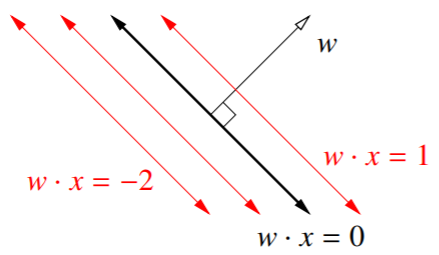
\includegraphics[width=0.5\textwidth]{CS189_Lec_02/lecture_2_signed_distance.png}
  \caption{A picture of a gull.}
\end{figure}


\textbf{If $w$ is a unit vector, then $w \cdot x + \alpha$ is the signed distance from $x$ to $H$. Why is that??}

First, we'll consider the case $w \cdot x = 0$. Consider any point $X_i$, the dot product $X_i \cdot w$ (the same as $w \cdot X_i$), indicates how much of $X_i$ is pointing to the same direction of $w$, and since $w$ is a unit vector, $X_i \cdot w = \Vert X_i \Vert cos \theta$, which, as the diagram below shows, is the \textbf{signed} distance from the hyperplane $H: {x: w \cdot x = 0}$.\newline

You can picture $w \cdot x = c$ as $w \cdot x + \alpha = 0$, where $\alpha = -c$. And as you can see from the red lines in the diagram, the lines move with respect to what value $\alpha$ is. So $w \cdot x + \alpha$ is really the signed distance from $x$ to $H$. Moreover, the distance from $H$ to the origin is $\alpha$.















\chapter{Lecture 3: Perceptron Learning; Maximum Margin Classifiers}
\section{Maximum Margin Classifier}
The \underline{margin} of a linear classifier is the distance from the decision boundary to the nearest sample. \newline\newline

Insert diagram here.\newline\newline

\textbf{And a "Maximum Margin Classifier" means we are making the margin as big as possible, } by enforcing the constraints \newline
\centerline{$y_i(\bm{w} \cdot X_i + \alpha) \geq 1 \quad \forall i \in [1,n]$}\newline\newline

Note that here we are still assigning $y_i = -1, 1$.

And by changing the right hand side to be 1, all the sample points can only at most touch the two dotted lines.

Notice that the right-hand side is a 1, rather than a 

Why $w$ now is impossible to be set to 0 is because if $w=0$, $X_i$ can be at any position, thus violates the constraint of setting a maximum margin.

Recall from Lecture 2: If $\Vert w \Vert = 1$, i.e., $w$ is a unit vector, signed distance from hyperplane to $X_i$ is $w \cdot x + \alpha$. \newline

Otherwise, we normalize the expression to get a unit weight vector\newline
$\begin{aligned}
	w \cdot x + \alpha &= 0 \\
    \frac{w}{\Vert w \Vert} \cdot x + \frac{\alpha}{\Vert w \Vert} &= 0 \\
\end{aligned}$
And by using this, the constraint now becomes:\newline
\centerline{$y_i(\frac{w}{\Vert w \Vert} \cdot x + \frac{\alpha}{\Vert w \Vert}) \geq \frac{1}{\Vert w \Vert}$}

So There is a slab of width $\frac{2}{|w|}$ containing no sample points [with the hyperplane running along its middle]\newline

So to maximize the margin, we have to minimize $\Vert w \Vert$. Hence the optimization problem becomes:\\
\framebox{Find $w$ and $\alpha$ that minimizes $\Vert w \Vert^2$ \newline
subject to $y_i(X_i \cdot w + \alpha) \geq 1 \quad$ for all $i \in [1,n]$}

\chapter{DLB - Chapter 3: Probability and Information Theory}

\section{Marginal Probability}
Sometimes we know the probability distribution over a set of variables and we want t know the probability distribution over just a subset of them. And the probability distribution over the subset is known as the \textit{marginal probability distribution}.\newline

For instance, suppose we have discrete random variables $X$ and $Y$, and we know $P(X,Y)$.\newline
We can find $P(X)$ with the \textit{sum rule}:\newline
    \centerline{$\forall x \in X, P(X=x) = \sum_y P(X=x,Y=y)$}\newline

For continuous variables, we need to use integration instead of summation:\newline
    \centerline{$p(x) = \int p(x,y)dy$}\newline

\section{Conditional Probability}
The probability of some event, given that some other event has happened, is called
\textit{conditional probability}. We denote the conditional probability that $Y=y$ given $X=x$ as $P(Y=y | X=x)$. which can be computed with the formula:\newline
    \centerline{$P(Y=y | X =x ) = \frac{P(Y=y,X=x)}{P(X=x)}$}\newline

\section{The Chain Rule of Conditional Probabilities}
Any joint probability distribution over many random variables may be decomposed into conditional distributions over only one variable:\newline
    \centerline{$P(X_1,...,X_n) = P(X_1)\prod_{i=2}^{n} P(X_i|X_1,...,X_{i-1})$}\newline

$\begin{aligned}
    P(X_1,...,X_n) &= P(X_n | X_1, ..., X_{n-1}) P(X_1, ..., X_{n-1}) \\
    &= P(X_n | X_1, ..., X_{n-1}) P(X_{n-1} | X_1, ..., X_{n-2}) P(X_1, ..., X_{n-2}) \\
    &= P(X_n | X_1, ..., X_{n-1}) P(X_{n-1} | X_1, ..., X_{n-2}) P(X_{n-2} | X_1, ..., X_{n-3}) P(X_1, ..., X_{n-3}) \\
    &= ... \\
    &= P(X_1)\prod_{i=2}^{n} P(X_i|X_1,...,X_{i-1})
\end{aligned}$

For example,\newline
\begin{itemize}
    \item $P(a,b,c) = P(a|b,c)P(b,c)$
    \item $P(b,c) = P(b|c)P(c)$
    \item $P(a,b,c) = P(a|b,c)P(b|c)P(c)$
\end{itemize}

\section{Independence and Conditional Independence}
Two random variables are \textbf{\textit{independent}} if their probability distribution can be expressed as a product of two factors, one involving only $X$ and one involving only $Y$:\newline\newline
\centerline{$\forall x \in X, y \in Y, p(X=x, Y=y) = p(X=x)p(Y=y)$}\newline\newline
Two random variables $X$ and $Y$ are conditionally independent given a random variable $Z$ if the conditional probability distribution over $X$ and $Y$ factorizes in this way for every value of $Z$:\newline\newline
\centerline{$\forall X \in x, Y \in y, z \in Z, p(X=x, Y=y | Z = z) = p(X=x | Z=z)p(Y=y | Z=z)$}\newline\newline
We can denote independence and conditional independence with compact notation: $X \perp Y$, means that $X$ and $Y$ are independent, while $X \perp Y | Z$ means that $X$ and $Y$ are conditionally independent given $Z$.\newline

\section{Expectation, Variance and Covariance}
The \textbf{\textit{expectation}} or \textbf{\textit{expected value}} of some function $f(x)$ with respect to a probability distribution $P(x)$ is the average or mean value that $f$ takes on when $x$ is drawn from P. Simply speaking, it means we are finding out if we're choosing different $x$ from $P$, then calculate $f(x)$, what's the average of $f(x)$.\newline

\noindent For discrete variables this can be computed with a summation:\newline\newline
\centerline{$\mathbb{E}_{X~P}[f(x)] = \sum_x P(x)f(x)$}\newline

\noindent while for continuous variables, it is computed with an integral:\newline\newline
\centerline{$\mathbb{E}_{X~P}[f(x)] = \int p(x)f(x)dx$}\newline

\noindent We can also simply write the name of the random variable that the expectation is over, as in $\mathbb{E}_X[f(x)]$. We may also omit the subscript entirely, as in $\mathbb{E}[f(x)]$.\newline

\noindent Expectations are linear, for example,\newline\newline
\centerline{$\mathbb{E}_X[\alpha f(x) + \beta g(x)] = \alpha \mathbb{E}_X[f(x)] + \beta \mathbb{E}_X[g(x)]$}\newline
when $\alpha$ and $\beta$ are not independent on $x$.\newline

\noindent The \textbf{\textit{variance}} gives a measure of how much the values of a function of a random variable $X$ vary as we sample different values of $x$ from its probability distribution:\newline\newline
\centerline{$\text{Var}(f(x)) = \mathbb{E}[(f(x) - \mathbb{E}[f(x)])^2]$}

\noindent As you can see, what $\text{Var}(f(x))$ is doing is it compares every $(f(x)$ with $\mathbb{E}[f(x)])$, but since that value can be positive or negative, so if calculate the average, we may get near to zero variance even though the values of the function varies a lot, so we square it.\newline

\noindent When the variance is low, the values of $f(x)$ cluster near their expected value. The square root of the variance is known as \textbf{\textit{standard deviation}}.\newline

\noindent The \textbf{\textit{covariance}} gives some sense of how much two values are linearly related to each other, as well as the scale of these variables:\newline\newline
\centerline{$\text{Cov}[f(x),g(y)]=\mathbb{E}[(f(x)-\mathbb{E}[f(x)])(g(y)-\mathbb{E}[g(y)])]$}\newline

\begin{itemize}
    \item High absolute values of the covariance mean that the values change very much and are both far from their respective means at the same time.
    \item If the sign of the covariance is positive, then both variables tend to take on relatively high values simultaneously.
    \item If the sign of the covariance is negative, then one variable tends to take on a relatively high value at the times that the other takes on a relatively low value and vice versa.
\end{itemize}
Other measures such as \textbf{\textit{correlation}} normalize the contribution of each variable in order to measure only how much the variables are related, rather than also being affected by the scale of the separate variables.\newline

\noindent The notions of covariance and dependence are related, but are in fact distinct concepts. They are related because two variables that are independent have zero covariance, and two variables that have non-zero covariance are dependent.\newline

\noindent However, independence is a distinct property from covariance. For two variables to have zero covariance, there must be no linear dependence between them. 

Independence is a stronger requirement than zero covariance, because independence also excludes nonlinear relationships. It is possible for two variables to be dependent but have zero covariance.

For example, suppose we first sample a real number $x$ from a uniform distribution over the interval $[-1, 1]$. We next sample a rando variable $s$. With probability $\frac{1}{2}$, we choose the value of $s$ to be 1. Otherewise, we choose the value of $s$ to be -1. We can then generate a random variable $y$ by assigning $y=sx$. Clearly, $x$ and $y$ are not independent, because $x$ completely determines the magnitude of $y$. However, $\text{Cov}(x,y)=0$.





\chapter{Machine Learning Basics}

\section{Learning Algorithms}
A machine learning algorithm is an algorithm that is able to learn from data. But what do we mean by learning?

\begin{quotation}
\noindent Mitchell (1997): \textit{"A computer is said to learn from experience $E$ with respect to some class of tasks $T$ and performance measure $P$, if its performance at tasks in $T$, as measured by $P$, improves with experience $E$."}
\end{quotation}

\subsection{The Task, $T$}
\noindent If we want a robot to be able to walk, then walking is the task. We could program the robot to learn to walk, or we could attempt to directly write a program that specifies how to walk manually.\newline

\noindent Machine learning tasks are usually described in terms of how the machine learning system should process an \textit{\textbf{example}}. An \textbf{\textit{example}} is a collection of \textbf{\textit{features}} that have been quantitatively measured from some object or event that we want the machine learning system to process. 

\noindent We typically represent an \textbf{\textit{example}} as a vector $x \in \mathbb{R}^n$ where each entry $x_i$ of the vector is another \textbf{\textit{feature}}. For example, the features of an image are usually the values of the pixels in the image.\newline

\noindent Some of the most common machine learning tasks include the following:\newline
\begin{itemize}
	\item Refer to Deep Learning Book's section 5.1.1, page 100-102
\end{itemize}

\subsection{The Performance Measure, $P$}
\noindent For tasks such as classification, classification with missing inputs, and transcription, we often measure the \textbf{\textit{accuracy}} of the model. Accuracy is just the proportion of examples for which the model produces the correct output. We can also obtain equivalent information by measuring the \textbf{\textit{error rate}}, the proportion of examples for which the model produce an incorrect output. We often refer to the error rate as the expected 0-1 loss. The 0-1 loss on a particular example is 0 if it is correctly classified and 1 if it is not. \newline

\noindent For tasks such as density estimation, it does not make sense to measure accuracy, error rate, or any other kind of 0-1 loss. Instead, we must use a different performance metric that gives the model a continuous-valued score for each example. The most common approach is to report the average log-probability the model assigns to some examples.\newline

\noindent Usually we are interested in how well the machine learning algorithm performs on data that it has not seen before, since this determines how well it will work when deployed in the real world. We therefore evaluate these performance measures using a \textbf{\textit{test set}} of data that is separate from the data used for training the machine learning system.\newline

\noindent In some cases, this is because it is difficult to decide what should be measured. For example, when performing a transcription task, should we measure the accuracy of the system at transcribing entire sequences, or should we use a more fine-grained performance measure that gives partial credit for getting some elements of the sequence correct? When performing a regression task, should we penalize the system more if it frequently medium-sized mistakes or if it rarely makes very large mistakes? These kinds of design choices depend on the application.\newline

\noindent In other cases, we know what quantity we would ideally like to measure, but measuring it is impractical. For example, this arises frequently in the context of density estimation. Many of the best probabilistic value assigned to a specific point in space in many such models is intractable. In these cases, one must design an alternative criterion that still corresponds to the design objectives, or design a good approximation to the desired criterion.\newline

\subsection{The Experience, $E$}
\noindent Machine learning algorithms can be broadly categorized as \textbf{\textit{unsupervised}} or \textbf{\textit{supervised}} by what kind of experience they are allowed to have during the learning process.\newline

\noindent Most of the learning algorithms in this book can be understood as being allowed to experience an entire \textbf{\textit{dataset}}. A dataset is a collection of many examples, as defined in Sec. 15.1.1. Sometimes we will also call examples \textbf{\textit{data points}}.\newline

\noindent One of the oldest datasets studied by statisticians and machine learning researchers is the Iris dataset (Fisher, 1936). It is a collection of measurements of different parts of 150 iris plants. Each individual plant corresponds to one example. The features within each example are the measurements of each of the parts of the plant: the sepal length, sepal width, petal length and petal width. The dataset also records which species each plant belonged to. Three different species are represented in the dataset.\newline

\noindent \textbf{\textit{Unsupervised learning algorithms}} experience a dataset containing many features, then learn useful properties of the structure of this dataset. In the context of deep learning, we usually want to learn the entire probability distribution that generated a dataset, whether explicitly as in density estimation or implicitly for tasks like synthesis or denoising. Some other unsupervised learning algorithms perform other roles, like clustering, which consists of dividing the dataset into clusters of similar examples.\newline

\noindent \textbf{\textit{Supervised learning algorithms}} experience a dataset containing features, but each example is also associated with a label or target. For example, the Iris dataset is annotated with the species of each iris plant. A supervised learning algorithm can study the Iris dataset and learn to classify iris plants into three different species based on their measurements.\newline

\noindent Roughly speaking, unsupervised learning involves observing several examples of a random vector $x$, and attempting to implicitly or explicitly learn the probability distribution $p(x)$, or some interesting properties of that distribution, while supervised learning involves observing several examples of a random vector $x$ and an associated value or vector $y$, and learning to predict $y$ from $x$, usually by estimating $p(y|x)$. The term \textbf{\textit{supervised learning}} originates from the view of the target $y$ being provided by an instructor or teacher who shows the machine learning system what to do. In \textbf{\textit{unsupervised learning}}, there is no instructor or teacher, and the algorithm must learn to make sense of the daata without this guide.\newline

\textbf{\textit{Unsupervised learning}} and \textbf{\textit{supervised learning}} are not formally defined terms. The lines between them are often blurred. Many machine learning technologies can be used to perform both tasks. For example, the chain rule of probability states that for a vector $x \in \mathbb{R}^n$, the joint distribution can be decomposed as\newline\newline
\centerline{$p(x) = \prod_{i=1}^{n} p(x_i | x_1, ..., x_{i-1})$}\newline\newline

This decomposition means that we can solve the ostensibly unsupervised problem of modeling $p(x)$ by splitting it into $n$ supervised learning problems. Alternatively, we can solve the supervised learning problem of learning $p(y|x)$ by using traditional unsupervised learning technologies to learn the joint distribution $p(x,y)$ and inferring\newline\newline
\centerline{$p(y|x)=\frac{p(x,y)}{\sum_{y'}p(x,y')}$}\newline

\noindent Though unsupervised learning and supervised learning are not completely formal or distinct concepts, they do help to roughly categorize some of the things we do with machine learning algorithms. Traditionally, people refer to regression, classification and structured output problems as supervised learning. Density estimation in support of other tasks is usually considered unsupervised learning.\newline

\noindent Other variants of the learning paradigm are possible. For example, in semisupervised learning, some examples include a supervision target but others do not. In multi-instance learning, an entire collection of examples is labeled as containing or not containing an example of a class, but the individual members of the collection are not labeled. For a recent example of multi-instance learning with deep models, see Kotzias et al. (2015).\newline

\noindent Some machine learning algorithms do not just experience a fixed dataset. For example, reinforcement learning algorithms interact with an environment, so there is a feedback loop between the learning system and its experiences. Such algorithms are beyond the scope of this book. Please see Sutton and Barto (1998) or Bertsekas and Tsitsiklis (1996) for information about reinforcement learning, and Mnih et al. (2013) for the deep learning approach to reinforcement learning.\newline

\noindent Most machine learning algorithms simply experience a dataset. A dataset can be described in many ways. In all cases, a dataset is a collection of examples, which are in turn collections of features.\newline

\noindent One common way of describing a dataset is with a \textbf{\textit{design matrix}}. A design matrix is a matrix containing a different example in each row. Each column of the matrix corresponds to a different feature. For instance, the Iris dataset contains 150 examples with four features for each example. This means we can represent the dataset with a design matrix $\mathbb{X} \in \mathbb{R}^{150x4}$, where $\mathbb{X}_{i,1}$ is the sepal length of plant $i$, $\mathbb{X}_{i,2}$ is the sepal width of plant $i$, etc. We will describe most of the learning algorithms in this book in terms of how they operate on design matrix datasets.\newline

\noindent Of course, to describe a dataset as a design matrix, it must be possible to describe 



\section{Example: Linear Regression}
Linear regression solves a regression problem. In other words, the goal is to build a system that can take a vector $x \in \mathbb{R}^n$ as input and predict the value of a scalar $y \in \mathbb{R}$ as its output. In the case of linear regression, the output is a linear function of the input. Let $\hat{y}$ be the value that our model predicts $y$ should take on. We define the output to be\newline
    \centerline{$\hat{y}= w^T x $}\newline
where $w \in \mathbb{R}^n$ is a vector of \textit{parameters}.\newline

We can think of $w$ as a set of \textit{weights} that determine how each feature affects the prediction.\newline

We thus have a definition of out task $T$: to predict $y$ from $\mathbf{x}$ by outputting $\hat{y}=\mathbf{w}^T\mathbf{x}$.\newline

Now we need a definition of our performance measure, $P$. Suppose that we have a design matrix of $m$ example inputs that we will not use for training, only for evaluating how well the model performs. We also have a vector of regression targets providing the correct value of $y$ for each of these examples. 

\chapter{Deep Feedforward Networks}
The goal of a feedforward network is to approximate some function $f^*$. For example, for a classifier, $y=f^*(x)$ maps an input $x$ to a category $y$. A feedforward network defines a mapping $y=f(x;\theta)$ and learns the value of $\theta$ that result in the best function approximation.\newline

\noindent These models are called \textit{feedforward} because information flows through the function being evaluated from $x$, through the intermediate computations used to define $f$, and finally to the output $y$. There are no \textit{feedback} connections in which outputs of the model are fed back into itself. When feedforward neural networks are extended to include  feedback connections, they are called \textit{recurrent neural networks}.\newline

\noindent Feedforward neural networks are called \textit{networks} because they are typically represented by composing together many different functions. The model is associated with a directed acyclic graph describing how the functions are composed together. For example, we might have three functions $f^{(1)}$, $f^{(2)}$, and $f^{(3)}$ connected in a chain, to form $f(x) = f^{(3)}(f^{(2)}(f^{(1)}(x)))$. These chain structures are the most commonly used structures of neural networks. In this case, $f^{(1)}$ is called the \textit{first layer of the network}, $f^{(2)}$ is called the \textit{second layer}, and so on. The overall length of the chain gives the \textit{depth} of the model. The final layer of a feedforward network is called \textit{output layer}.\newline

\noindent During neural network training, we drive $f(x)$ to match $f^*(x)$. The training data provides us with noisy, approximate examples of $f^*(x)$ evaluated at different training points. Each example $x$ is accompanied by a label $y \approx f^*(x)$. The training examples specify directly what the output layer must do at each point $x$; it must produce a value that is close to $y$. The behavior of other layers is not directly specified by the training data. The learning algorithm must decide how to use those layers to produce the desired output, but the training data does not say what each individual layer should do. Instead, the learning algorithm must decide how to use these layers to best implement an approximation of $f^*$. Because the training data does not show the desired output for each of these layers, these layers are called \textit{hidden layers}.\newline

\noindent Each hidden layer of the network is typically vector-valued. The dimensionality of these hidden layers determines the \textit{width} of the model. Each element of the vector may in interpreted as playing a role analogous to a neuron. Rather than thinking of the layer as consisting of many \textit{units} that act in parallel, each representing a vector-to-scalar function. Each unit resembles a neuron in the sense that it receives input from other units and computes its own activation value. The idea of using many layers of vector-valued representation is drawn from neuroscience. The choice of the functions $f^{(i)}(x)$ used to compute these representations is also loosely guided by neuroscientific observations about the functions that biological neurons compute. However, it is best to think of feedforward networks as function approximation machines that are designed to achieve statistical generalization, occasionally drawing some insights from what we know about the brain, rather than as models of brain function.\newline

\noindent One way to understand feedforward networks is to begin with linear models and consider how to overcome their limitations. Linear models, such as logistic regression and linear regression, are appealing because they may be fit efficiently and reliably, either in closed form or with convex optimization. Linear models also have the obvious defect that the model capacity is limited to linear functions, so the model cannot understand the interaction between any two input variables.\newline

\noindent To extend linear models to represent nonlinear functions of $x$, we can apply the linear model not to $x$ itself but to a transformed input $\phi(x)$, where $\phi$ is a nonlinear transformation. Equivalently, we can apply the kernel trick described in (Deep Learning Book's Section 5.7.2), to obtain a nonlinear learning algorithm based on implicitly applying the $\phi$ mapping. We can think of $\phi$ as providing a set of features describing $x$, or as providing a new representation for $x$.

\noindent The question is then how to choose the mapping $\phi$:
\begin{enumerate}
	\item Use a very generic $\phi$, such as the infinite-dimensional $\phi$ that is implicitly used by kernel machines based on the RBF kernel.\newline
    	\begin{itemize}
    		\item If $\phi(x)$ is of high enough dimension, we can always have enough capacity to fit the training set, but generalization to the test set often remains poor.
            \item Very generic feature mappings are usually based only on the principle of local smoothness and do not encode enough prior information to solve advanced problems.
    	\end{itemize}
    \item Manually engineer $\phi$\newline
    	\begin{itemize}
    		\item Until the advent of deep learning, this was the dominant approach.
            \item This approach requires decades of human effort for each separate task, with peactitioners specializing in different domains such as speech recognition or computer vision, and with little transfer between domains.
    	\end{itemize}
    \item Learn $\phi$.\newline
    	\begin{itemize}
    		\item In this approach, we have a model $y=f(x; \theta, w) = \phi(x; \theta)^Tw$
    	\end{itemize}
\end{enumerate}

\chapter{Convolutional Networks}
Convolutional networks are simply neural networks that use convolution in place of general matrix multiplication in at least one of their layers.

\section{The Convolution Operation}
In its most general form, convolution is an operation on two functions of a real-valued argument.\newline

\noindent Suppose we are tracking the location of a spaceship with a laser sensor. Our laser sensor provides a single output $x(t)$, the position of the spaceship at time $t$. Both $x$ and $t$ are real-valued, i.e., we can get a different reading from the laser sensor at any constant in time.\newline

\noindent Now suppose that our laser sensor is somewhat noisy. To obtain a less noisy estimate of the spaceship's position, we would like to average together several measurements. Of course, more recent measurements are more relevant, so we will want this to be a weighted function $w(a)$, where $a$ is the age of a measurement. We can do this a weighting average operation at every moment, we obtain a new function $s$ providing a smoothed estimate of the position of the spaceship:\newline\newline
    \centerline{$s(t) = \int [x(a)][w(t-a)]da$}\newline\newline
\noindent This operation is called \textit{convolution}. The convolution operation is typically denoted with an asterisk:\newline
    \centerline{$s(t) = (x * w)(t)$}\newline

In our example, $w$ needs to be a valid probability density function, or the output is not a weighted average. Also, $w$ needs to be 0 for all negative arguments, or it will look into the future, which is presumably beyond our capabilities. These limitations are particular to our example though. In general, convolution is defined for any functions for which the above integral is defined, and may be used for other purposes besides taking weighted averages.\newline

\noindent In convolutional network terminology, the first argument (in this example, the function $x$) to the convolution is often referred to as the \textit{input} and the second argument (in this example, the function $w$) as the \textit{kernel}. The output is sometimes referred to as the \textit{feature map}.\newline

\noindent In our example, the idea of a laser sensor that can provide measurements at every instant in time is not realistic. Usually, when we work with data on a computer, time will be discretized, and our sensor will provide data at regular intervals. In our example, it might be more realistic to assume that our laser provides a measurement once per second. The time index $t$ can then take on only integer values. If we now assume that $x$ and $w$ are defined only on integer $t$, we can define the discrete convolution:\newline\newline
    \centerline{$s(t) = (x * w)(t) = \sum_{a=-\infty}^{\infty}[x(a)][w(t-a)]$}\newline\newline
In machine learning applications, the input is usually a multidimensional array of parameters that are adapted by the learning algorithm. We will refer to these dimensional arrays as tensors. Because each element of the input and kernel must explicitly stored separately, we usually assume that these functions are zero everywhere but the finite set of points for which we store the values. This means that in practice we can implement the infinite summation as a summation over a finite number of array elements.\newline

\noindent Finally, we often use convolutions over more than one axis at a time. For example, if we use a two-dimensional image $I$ as our input, we probably also want to use a two-dimensional kernel $K$:\newline\newline
    \centerline{$S(i,j)=(I*K)(i,j)=\sum_m \sum_n I(m,n)K(i-m,j-n)$}\newline\newline
    
Here, the input is $I$, the kernel is $K$.\newline

Convolution is commutative, meaning we can equivalently write:\newline\newline
    \centerline{$S(i,j)=(K*I)(i,j)=\sum_m \sum_n K(m,n)I(i-m,j-n)=I(i-m,j-n)K(m,n)$}\newline\newline

Usually the latter formula is more straightforward to implement in a machine learning library, because there is less variation in the range of valid values of $m$ and $n$.\newline

The commutative property of convolution arises because we have \textit{flipped} the kernel relative to the input, in the sense that as $m$ increases, the index into the input increases, but the index into the kernel decreases. The only reason to flip the kernel is to obtain the commutative property. While the commutative property is useful for writing proofs, it is not usually an important property of a neural network implementation.\newline

\noindent Instead, many neural network libraries implement a related function called the \textbf{\textit{cross-correlation}}, which is the same as convolution but without flipping the kernel:\newline\newline
    \centerline{$S(i,j)=(I*K)(i,j)=\sum_m \sum_n I(i+m,j+n)K(m,n)$}\newline\newline
    
Many machine learning libraries implement cross-correlation but call it convolution. 

blah blah blah

\subsection{Convolution and Correlation}
http://www.cs.umd.edu/~djacobs/CMSC426/Convolution.pdf

Convolution and correlation have two key features:
\begin{itemize}
	\item \textit{shift-invariant}: we perform the same operation at every point in the image
    \item \textit{linear}: the operation is linear, that is, we replace every pixel with a linear combination of its neighbors.
\end{itemize}

These two properties make these operations very simple; it's simpler if we do the same thing everywhere, and linear operations are always the simplest ones.

\subsubsection{Example:}
One of the simplest operations that we can perform with correlation is local averaging, which we replace every pixel in a 1D image by the average of that pixel and its two neighbors. Suppose we have an image $I$ equal to:

\begin{table}[ht]
\centering
\label{my-label}
\begin{tabular}{|l|l|l|l|l|l|l|l|l|l|}
\hline
5 & 4 & 2 & 3 & 7 & 4 & 6 & 5 & 3 & 6 \\ \hline
\end{tabular}
\caption{image $I$}
\end{table}

Averaging is an operation that takes an image as input, and produces a new image as output. When we average the fourth pixel, for instance, we replace the value 3 with the average of 2,3 and 7. That is, if we call the new image that we produce $J$ we can write:\newline
    \centerline{$J(4) = [I(3)+I(4)+I(5)]/3 = 4$}\newline
Notice that every pixel in the new image depends on the pixels in the old image. Averaging like this is shift-invariant, because we perform the same operation at every pixel. Every new pixel is the average of itself and its two neighbors. Averaging is linear because every new pixel is a linear combination of the old pixels. This example illustrates another property of all correlation and convolution that we will consider: The output image at a pixel is based on only a small neighborhood of pixels around it in the input image.


\textbf{Boundaries:} We still haven't fully described correlation, because we haven't said what to do at the boundaries of the image. What is $J(1)$? There is no pixel on its left to include in the average, i.e., $I(0)$ is not defined. There are four common ways of dealing with this issue:
\begin{itemize}
    \item The first way is to image that $I$ is part of an infinitely long image which is zero everywhere except where we have specified. So we can say:\newline\newline
        \centerline{$J(1)=[I(0)+I(1)+I(2)]/3=(0+5+4)/3=3$}\newline
        \begin{table}[h]
        \centering
        \label{my-label-1}
        \begin{tabular}{|l|l|l|l|l|l|l|l|l|l|l|l|l|l|l|l|}
        \hline
        . & . & .& 5 & 4 & 2 & 3 & 7 & 4 & 6 & 5 & 3 & 6 & . & . & .\\ \hline
        \end{tabular}
        \caption{image $I$}
        \end{table}
        
    \item The second way is to also imagine that $I$ is part of an infinite image, but to extent it using the first and last pixels in the image. So we can say: \newline\newline
          \centerline{$J(1)=[I(0)+I(1)+I(2)]/3=(5+5+4)/3=4.66666$}\newline\newline    
        \begin{table}[h]
        \centering
        \label{my-label-2}
        \begin{tabular}{|l|l|l|l|l|l|l|l|l|l|l|l|l|l|l|l|l|l|l|l|}
        \hline
        . &. & . & 5 & 5 & 5 & 4 & 2 & 3 & 7 & 4 & 6 & 5 & 3 & 6 & 6 & 6 & . & . & .\\ \hline
        \end{tabular}
        \caption{image $I$}
        \end{table}
        
    \item The third way is to imagine the image as being like a circle, so that the pixel values repeat over and over again. So we would have\newline\newline
        \centerline{$J(1)=[I(0)+I(1)+I(2)]/3=(6+5+4)/3=5$}
    \item Finally, we can simply say that the image is undefined beyond the values that we have been given. In that case, we cannot compute any average that uses these undefined values, so $J(1)$ and $J(10)$ will be undefined, and $J$ will be smaller that $I$.
\end{itemize}

These four methods have different advantages and disadvantages. If we imagine that the image we are using is just a small window on the world, and we want to use values outside the boundary that are most similar to the values that we would have obtained if we'd taken a bigger picture, then the second approach probably makes the most sense. That is, if we had to guess at the value of $I(0)$, even though we can't see it, the value we can see in $I(1)$ is probably a pretty good guess.

\subsubsection{Correlation as a Sliding, Windowed Operation}
We're now going to look at the same averaging operation in a slightly different way which is more graphical, and perhaps more intuitive to generalize. In averaging, for a specific pixel we multiply it and its neighbors by 1/3 each, and then add up the three resulting numbers. The numbers we multiply, (1/3, 1/3, 1/3) form a \textit{filter}. This particular filter is called a \textit{box} filter. We can think of it as a 1x3 structure that we slide along the image. At each position, we multiply each number of the filter by the image number that lies underneath it, and add these all up. The result is a new number corresponding to the pixel that is underneath the center of the filter.\newline

We continue to do the sliding until we have produced every pixel in $J$. With this view of correlation, we can define a new averaging procedure by just defining a new filter. For example, suppose instead of averaging a pixel with its immediate neighbors, we want to average each pixel with immediate neighbors and their immediate neighbors. We can define a filter as (1/5,1/5,1/5,1/5,1/5). Then we perform the same operation as above, but using a filter that is five pixels wide. The first pixel in the resulting image will then be: $J(1)=I(-1)/5+I(0)/5+I(1)/5+I(2)/5+I(3)/5=1+1+1+4/5+2/5=4.2$

\subsubsection{A Mathematical Definition for Correlation}
Suppose $F$ is a correlation filter, it will be convenient notationally to suppose that F has an odd number of elements, so we can suppose that as it shifts, its center is right on top of an element of $I$. So we say that $F$ has $2N+1$ elements, and that these are indexed from $-N$ to $N$, so that the center element of $F$ is $F(0)$. Then we can write:\newline\newline
    \centerline{$F \circ I(x) = \sum_{i=-N}^N F(i)I(x+i)$}\newline\newline
where the circle denotes correlation. With this notation, we can define a simple box filter as:\newline\newline
    \centerline{$F(i) = \left\{\begin{matrix}
1/3 & for & i = -1,0,1 \\ 
0 & for & i \neq -1,0,1
\end{matrix}\right.$}

\subsubsection{Constructing an Filter from a Continuous Function}
It is pretty intuitive what a reasonable averaging filter should look like. Now we want to start to consider more general strategies for constructing filters. It commonly occurs that we have in mind a continuous function that would make a good filter, and we want to come up with a discrete filter that approximates this continuous function. Some reasons for thinking of filters first as continuous functions will be given when we talk about the Fourier transform. But in the mean time we'll give an example of an important continuous function used for image smoothing, the Gaussian.

A one-dimensional Gaussian is:\newline
    \centerline{$G(x) = \frac{1}{\sigma \sqrt{2 \pi}} exp\left ( \frac{-(x - \mu)^2}{2\sigma^2} \right )$}\newline\newline
This is also known as a Normal distribution. Here $\mu$ is the mean value, and $\sigma$ is the variance.

The mean, $\mu$, gives the location of the peak of the function. The parameter $\sigma$ controls how wide the peak is. As $\sigma$ gets smaller the peak becomes narrower.

The Gaussian has a lot of very useful properties, some of which we'll mention later. 
\begin{itemize}
    \item When we use it as a filter, we can think of it as a nice way to average. The averaging filter that we introduced above replaces each pixel with the average of its neighbors. This means that nearby pixels all play an equal role in the average, and more distant pixels play no role.
    \item It is more appealing to use the Gaussian to replace each pixel with a weighted average of its neighbors. In this way, the nearest pixels influence the average more, and more distant pixels play a smaller and smaller role. This is more elegant, because we have a smooth and continuous change. We will show this more rigorously when we discuss the Fourier transform.
\end{itemize}

When we use a Gaussian for smoothing, we will set $\mu=0$, because we want each pixel to be the one that has the biggest effect on its new, smoothed value. So our Gaussian has the form:\newline\newline
    \centerline{$G_0(x) = \frac{1}{\sigma \sqrt{2 \pi}} exp\left ( \frac{-x^2}{2\sigma^2} \right )$}

$\sigma$ will serve as a parameter that allows us to control how much we smooth the image (that is, how big a neighborhood we use for averaging). The bigger $\sigma$ is, the more we smooth the image.

We now want to build a discrete filter that looks like a Gaussian. We can do this by just evaluating the Gaussian at discrete locations. That is, although $G$ is defined for any continuous value of $x$, we will just use its values at discrete locations (..., -3, -2, -2, 0, 1, 2, 3, ...). One way to think about this is that we are approximating our original, continuous function with a piecewise constant function, where the pieces are each one pixel wide.

However, we cannot evaluate $G$ at every integer location, because this would give s a filter that is infinitely long, which is impractical. Fortunately, as $x$ gets away from 0, the value of $G(x)$ will approach 0 pretty quickly, so it will be safe to ignore some values of $G(x)$, but a reasonable rule of thumb is to make sure we capture $99\%$ of the function. What we mean by this is that the sum of values in our filter will contain at least $0\%$ of what we would get in an infinitely long filter, that is, we choose $N$ so that:\newline\newline
    \centerline{$\frac{\sum_{-N}^{N}G(x)}{\sum_{-\infty}^{\infty}G(x)} > .99$}
    
There is one final point. An averaging filter should have all its elements add up to 1. This is what averaging means: if the filter elements don't add up to one, then we are not only smoothing the iamge, we are making it dimmer or brighter. The continuous Gaussian integrates to one (after all, it's a probability density function, and probabilities must add up to one), but when we sample it and truncate it, there is no guarantee that the values we get will still add up to one. So we must normalize our filter, meaning the elements of our filter will be calculate as:\newline\newline
    \centerline{$F(i) = \frac{G(i)}{\sum_{-N}^{N}G(x)}$ for $i=-N...N$}\newline

\subsubsection{Taking Derivatives with Correlation}
Averaging, or smoothing, is one of the most important things we can do with a filter. However, another very useful thing is taking a derivative. This allows us to measure how quickly an image is changing. Taking derivatives is something we usually think of doing with a continuous function. Technically, derivatives aren't even defined on a discrete image, because a derivative measures how quickly the image is changing over an interval, in the limit, as the interval becomes infinitely small. However, just as we were able to produce a discrete filter that was an approximation to a continuous Gaussian, we can discretely approximate a continuous derivative operator.

Intuitively, a derivative is found by taking the difference as we go from one part of a function to another. That is, it's the change in $y$ divided by the change in $x$. So it's natural that a derivative filter will look something like: (-1/2 0 1/2). When we apply this filter, we get $J(i) = [I(i+1)-I(i-1)]/2$. This is taking the change in $y$, that is, the image intensity, and dividing it by the change in $x$, the image position.

Let's consider an example. Suppose image intensity grows quadratically with position, so that $I(x)=x^2$. Then if we look at the intensities at positions 1,2,3,... they will look like:

\begin{table}[ht]
\centering
\label{my-label-3}
\begin{tabular}{|l|l|l|l|l|l|l|l|l|}
\hline
1 & 4 & 9 & 16 & 25 & 36 & . & . & . \\ \hline
\end{tabular}
\caption{image $I$}
\end{table}

If we filter this with a filter of the form (-1/2 0 1/2) we will get:
\begin{table}[ht]
\centering
\label{my-label-4}
\begin{tabular}{|l|l|l|l|l|l|l|l|l|}
\hline
1.5 & 4 & 6 & 8 & 10 & 12 & . & . & . \\ \hline
\end{tabular}
\caption{image $I$}
\end{table}

We know that the derivative of $I(x), dI/dx = 2x$. And sure enough, we have, for example, that $J(2)=4, J(3)=6, ...$ Notice that $J(1)$ is not equal to 2 because of the way we handle the boundary, by setting $I(0) = 1$ instead of $I(0) = 0$. So at the boundary, our image doesn't reflect $I(x) = x^2$.

We could just as easily have used a filter like (0 -1 1), which computes the expression: $J(i) = [I(i+1)-I(i)]/1$, or a filter (-1 1 0), which computes $J(i) = [I(i)-I(i-1)]/1$. These are all reasonable approximations to a derivative. One advantage of the filter (-1/2 0 1/2) is that it treats the neighbors of a pixel symmetrically.

\subsubsection{Matching with Correlation}
Part of the power of correlation is that we can use it, and related methods, to find locations in an image that are similar to a template. To do this, think of the filter as a template; we are sliding it around the image looking for a location where the template overlaps the images so that values in the template are aligned with similar values in the image.

First, we need to decide how to measure the similarity between the template and the region of the image with with which it is aligned. A simple and natural way to do this to measure the sum of the square of the differences between values in the template and in the image. This increases as the difference between the two increases. For the difference between the filter and the portion of the image centered at $x$, we can write this as:

$\begin{aligned}
    \sum_{i=-N}^{N}[F(i)-I(x+i)]^2 &= \sum_{i=-N}^{N}[F^2(i)+I^2(x+i)-2F(i)I(x+i)] \\
    &= \sum_{i=-N}^{N}[F^2(i)] + \sum_{i=-N}^{N}[I^2(x+i)] + 2\sum_{i=-N}^{N}[F(i)I(x+i)]
\end{aligned}$


As shown, we can break the Euclidean distance into three parts:
\begin{itemize}
    \item The first part depends only on the filter. This will be the same for every pixel in the image.
    \item The second part is the sum of squares of pixel values that overlap the filter.
    \item And the third part is twice the negative value of the correlation between $F$ and $I$.
\end{itemize}

We can see that, all things being equal, as the correlation between the filter and the image increases, the Euclidean distance between them decreases. This provides an intuition for using correlation to match a template with an image. Places where the correlation between the two is high tend to be locations where the filter and image match well.

This also shows one of the weaknesses of using correlation to compare a template and image. Correlation can also be high in locations where the image intensity is high, even if it doesn't match the template well. Here's an example. Suppose we correlate the filter

\begin{table}[ht]
\centering
\label{my-label-5}
\begin{tabular}{|l|l|l|}
\hline
3 & 7 & 5 \\ \hline
\end{tabular}
\end{table}

with the image:

\begin{table}[ht]
\centering
\label{my-label-6}
\begin{tabular}{|l|l|l|l|l|l|l|l|l|l|l|l|l|l|l|l|l|}
\hline
3 & 2 & 4 & 1 & 3 & 8 & 4 & 0 & 3 & 8 & 0 & 7 & 7 & 7 & 1 & 2\\ \hline
\end{tabular}
\end{table}

We get the following the result:

\begin{table}[ht]
\centering
\label{my-label-7}
\begin{tabular}{|l|l|l|l|l|l|l|l|l|l|l|l|l|l|l|l|l|}
\hline
40 & 43 & 39 & 34 & 64 & 85 & 52 & 27 & 61 & 65 & 59 & 84 & 105 & 75 & 38 & 27 \\ \hline
\end{tabular}
\end{table}

Notice that we get a high result (85) when we center the filter on the \textbf{\textit{sixth}} pixel, because (3,7,5) matches very well with (3,8,4). But, the highest correlation occurs at the thirteenth pixel, where the filter is matched to (7,7,7). Even though this is not as similar to (3,7,5), its magnitude is greater.

One way to overcome this is by just using the sum of square differences between the signals, as given above. This produces the result:

\begin{table}[ht]
\centering
\label{my-label-8}
\begin{tabular}{|l|l|l|l|l|l|l|l|l|l|l|l|l|l|l|l|l|}
\hline
25 & 26 & 26 & 41 & 29 & 2 & 59 & 54 & 34 & 26 & 78 & 13 & 20 & 32 & 61 & 38 \\ \hline
\end{tabular}
\end{table}

We can see that using Euclidean distance, (3,7,5) best matches the part of the image with pixel values (3,8,4). The next best match has values (0,7,7), but this is significantly worse.

Another option is to perform \textbf{\textit{normalized correlation}} by computing:\newline

\centerline{$\frac{\sum_{i=-N}^N [F(i)I(x+i)]}{\sqrt{\sum_{i=-N}^N [I(x+i)]^2} \sqrt{\sum_{i=-N}^N [F(i)]^2}}$}

This measure of similarity is similar to correlation, but it is invariant to scaling the template or a corresponding region in the image. If we scale $I(x-N)...I(x+N)$, by a single, constant factor, this will scale the numerator and denominator by the same amount. Consequently, for example, (3,7,5) will have the same normalized correlation with (7,7,7) that it would have with (1,1,1). When we perform normalized correlation between (3,7,5) and the above image we get:

\begin{table}[ht]
\centering
\label{my-label-9}
\begin{tabular}{|l|l|l|l|l|l|l|l|l|l|l|l|l|l|l|l|l|}
\hline
.946 & .877 & .934 & .73 & .81 & .989 & .64 & .59 & .78 & .835 & .61 & .931 & .95 & .83 & .57 & .988 \\ \hline
\end{tabular}
\end{table}

(not finished)

\subsection{Motivation}
Convolution leverages three important ideas that can help improve a machine learning system:
\begin{itemize}
	\item \textbf{sparse interaction}
    \item \textbf{parameter sharing}
    \item \textbf{equivariant representations}
\end{itemize}
Moreover, convolution provides a means for working with inputs of variable size.

\noindent \textbf{Traditional neural network layers} use matrix multiplication by a matrix of parameters with a separate parameter describing the interaction between each input unit and each output unit. This means that every output unit interacts with every input unit.

\noindent \textbf{Convolutional networks}, however, typically have \textbf{sparse interactions}. This is accomplished by making the kernel smaller that the input. For example, when processing an image, meaningful features such as edges with kernels that occupy only tens or hundreds of pixels. This means that we need to store fewer parameters, which both reduces the memory requirements of the model and improves its statistical efficiency.It also means that computing the output requires fewer operations.

\noindent These improvements in efficiency are usually quite large. If there are $m$ inputs and
$n$ outputs, then 
\begin{itemize}
	\item matrix multiplication requires $mxn$ parameters
    \item algorithms used in practice have $O(m \times n)$ runtime (per sample)
\end{itemize}
If we limit the number of connections each output may have to $k$, then the sparsely connected approach requires only $k \times n$ parameters and $O(k \times n)$ runtime. For graphical demonstration of sparse connectivity, check out the following figure:

\begin{figure}[H]
  \centering
  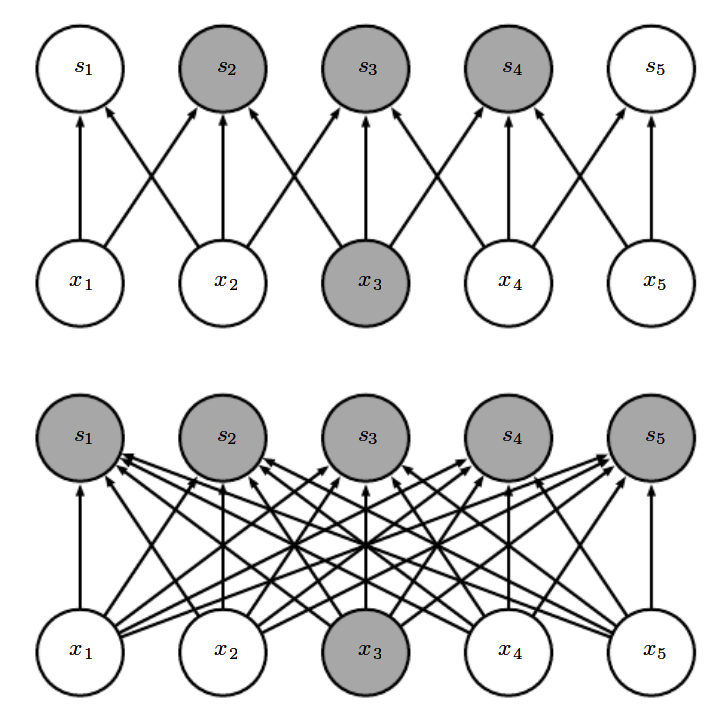
\includegraphics[width=0.5\textwidth]{Convolutional_Networks/sparse_connectivity_1.png}
  \caption{\textbf{Sparse Connectivity, view from below}: We highlight one input unit, $x_3$, and highlight the output units in $s$ that are affected by this unit. At the \textbf{\textit{top}}, when $s$ is formed by convolution with a kernel of width 3, only three inputs are affected by $x$. At the \textbf{\textit{bottom}}, when $s$ is formed by matrix multiplication, connectivity is no longer sparse, so all the outputs are affected by $x_3$.}
\end{figure}

\begin{figure}[H]
  \centering
  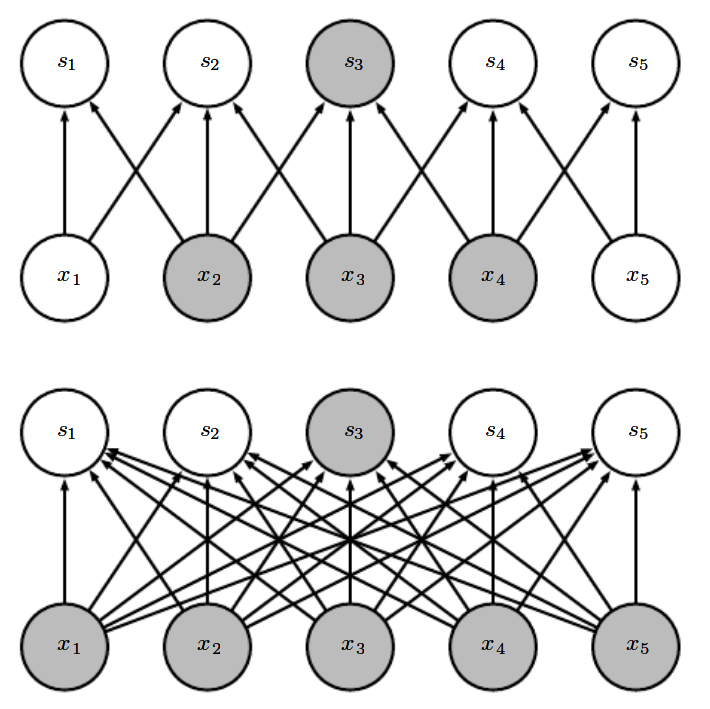
\includegraphics[width=0.5\textwidth]{Convolutional_Networks/sparse_connectivity_2.png}
  \caption{\textbf{Sparse Connectivity, view from above}: We highlight one output unit, $s_3$, and highlight the input units in $x$ that affect this unit. These units are known as the \textbf{receptive field} of $s_3$. At the \textbf{\textit{top}}, when $s$ is formed by convolution with a kernel of width 3, only three inputs affect $s_3$. At the \textbf{\textit{bottom}}, when $s$ is formed by matrix multiplication, connectivity is no longer sparse, so all the inputs affect $s_3$.}
\end{figure}

In a deeper convolutional network, units in the deeper layers may \textit{indirectly} interact with a larger portion of the input, as shown in the following figure. This allows the network efficiently describe complicated interactions between many variables by constructing such interaction from simple building blocks that each describe only sparse interactions.

\begin{figure}[h!]
  \centering
  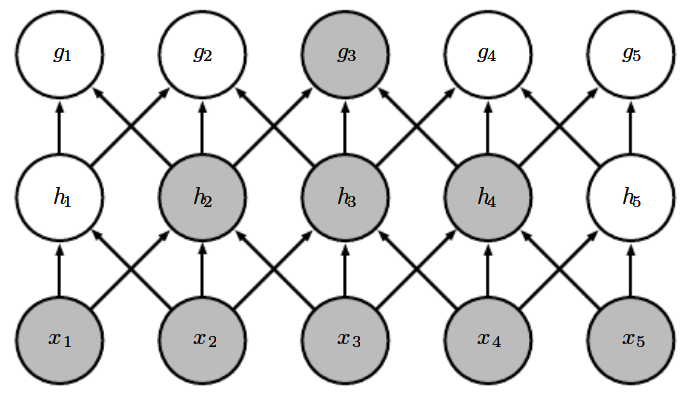
\includegraphics[width=0.5\textwidth]{Convolutional_Networks/sparse_connectivity_3.png}
  \caption{The receptive field of the units in the deeper layers of a convolutional network is larger than the receptive field of the units in the shallow layers. This effect increases if the network includes architectural features like \textit{strided} convolution or \textit{pooling}. This means that even though \textbf{\textit{direct}} connections in a convolutional net are very sparse, units in the deeper layers can be \textbf{\textit{indirectly}} connected to all or most of the input image.}
\end{figure}

\noindent \textbf{Parameter sharing} refers to using the same parameter for more than one function in a model. In a \textbf{traditional neural net}, each element of the weight matrix is used exactly once when computing the output of a layer. It is multiplied by one element of the input and then never revisited. As a synonym for parameter sharing, one can say that a network has \textbf{tied weights}, because the value of the weight applied to one input is tied to the value of a weight applied elsewhere. In a \textbf{convolutional neural net}, each member of the kernel is used at every position of the input (except perhaps some of the boundary pixels, depending on the design decisions regarding the boundary). Te parameter sharing used by the convolution operation means that rather than learning a separate set of parameters for every location, we learn only one set.

\noindent This does not affect the runtime of forward propagation - it is still $O(k \times n)$ - but it does further reduce the storage requirements of the model to $k$ parameters. Recall than $k$ is usually several orders of magnitude smaller than $m$. Since $m$ and $n$ are usually roughly the same size, $k$ is practically insignificant compared to $m \times n$. Convolution is thus dramatically more efficient than dense matrix multiplication in terms of the memory requirements and statistical efficiency. For a graphical depiction of how parameter sharing works, check out the following figure:

\begin{figure}[h!]
  \centering
  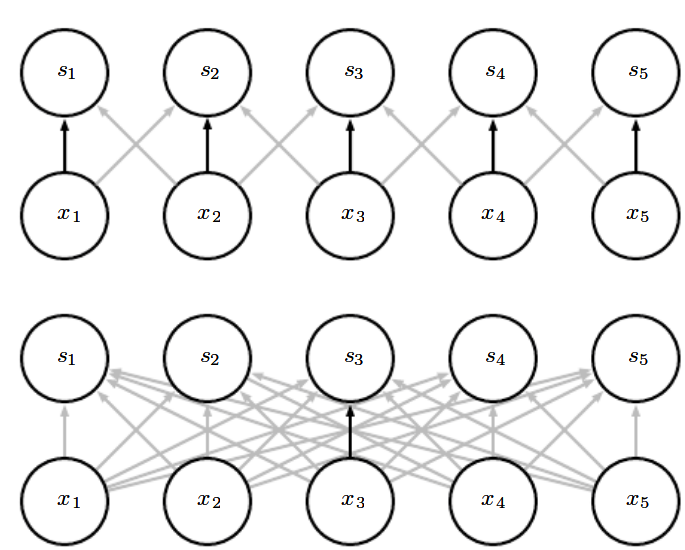
\includegraphics[width=0.5\textwidth]{Convolutional_Networks/parameter_sharing.png}
  \caption{\textbf{Parameter sharing}: Black arrows indicate the connections that use a particular parameter in two different models. At the \textbf{\textit{top}}, the black arrows indicate uses of the central element of a 3-element kernel in a convolutional model.}
\end{figure}

% Uncomment the following two lines if you want to have a bibliography. Please do not forget to add an entry to your bibliography and reference it by using the \cite{} command
%\bibliographystyle{alphadin}
%\bibliography{document}

% End of the document
\end{document}
